% =====================================================================
% Relatorio (versao acessivel) — Trocar o controlador PID de pitch por LSTM
% Compilar: pdflatex relatorio.tex (2x para sumario/referencias)
% =====================================================================
\documentclass[11pt,a4paper]{article}

\usepackage[utf8]{inputenc}
\usepackage[T1]{fontenc}
\usepackage{lmodern}
\usepackage[brazil]{babel}
\usepackage[margin=2.5cm]{geometry}
\usepackage{graphicx}
\usepackage{booktabs}
\usepackage{amsmath}
\usepackage{amssymb}
\providecommand{\checkmark}{\ensuremath{\surd}}
\usepackage{float}
\usepackage{caption}
\usepackage{xcolor}
\usepackage{tikz}
\usetikzlibrary{arrows.meta,positioning,calc,fit}
\usepackage[colorlinks=true,linkcolor=blue!50!black,citecolor=blue!50!black,urlcolor=blue!50!black]{hyperref}

\captionsetup{font=small,labelfont=bf}
\graphicspath{{figuras/}}

\newcommand{\thetaref}{\theta_{\mathrm{ref}}}

\title{\textbf{Trocando o Controlador Clássico (PID) de um Avião\\
por uma Rede Neural (LSTM)}\\[2mm]
\large Imitação de um controlador PI por rede recorrente, com refinamento por DAgger e
análise de robustez}
\author{Kauê Martins de Souza\\[1mm]
\small Trabalho Final --- Estágio Docência\\
\small Orientação: Prof.\textsuperscript{a} Neusa Maria}
\date{Junho de 2026}

\begin{document}
\maketitle

\begin{center}
\small Material completo (código MATLAB/Simulink, dados e este relatório):
\url{https://github.com/gabimont/pitch_lstm}
\end{center}

\begin{abstract}
\noindent Todo avião precisa de um ``piloto automático'' que mantenha o nariz na
inclinação certa. Tradicionalmente isso é feito por um \textbf{controlador clássico}
(uma fórmula matemática bem conhecida, o PID). Neste trabalho, trocamos essa fórmula
por uma \textbf{rede neural} --- um programa de computador que \emph{aprende sozinho},
a partir de exemplos. Ensinamos a rede a \emph{imitar} o controlador clássico e depois
a colocamos para comandar o avião sozinha, comparando os dois. O resultado tem três
partes: (1)~quando treinada corretamente, a rede neural funciona tão bem quanto o
controlador clássico; (2)~a imitação simples, porém, não basta --- a rede precisou de
um treino extra (chamado \emph{DAgger}) para parar de ``balançar'' o avião; e
(3)~mapeamos onde a rede funciona e onde ela falha. A lição final, em uma frase:
\textbf{a rede neural só é confiável nas situações parecidas com as que ela viu durante
o treino}. Fora delas, ela piora --- mas, neste estudo, nunca a ponto de descontrolar
totalmente o avião.
\end{abstract}

\tableofcontents
\newpage

% =====================================================================
\section{O que estamos tentando fazer}
% =====================================================================

O problema é o controle de arfagem (\emph{pitch}) de uma aeronave: manter o ângulo
$\theta$ numa referência $\thetaref$, atuando no profundor. O laço mede $\theta$,
compara com $\thetaref$ e calcula o comando de deflexão --- tarefa classicamente
resolvida por um controlador \textbf{PID/PI}, com garantias de estabilidade e
desempenho bem estabelecidas. A pergunta deste trabalho é:

\begin{quote}
\emph{E se, no lugar dessa fórmula clássica, usássemos uma \textbf{rede neural} ---
um programa que aprende sozinho a partir de exemplos?}
\end{quote}

Redes neurais são flexíveis e estão por trás de muita tecnologia moderna (reconhecer
fotos, traduzir textos). A ideia aqui é ensinar uma rede a controlar o avião e medir,
com cuidado, \textbf{onde ela funciona, onde falha e por quê}. Tudo foi feito em
simulação, no programa MATLAB/Simulink.

% =====================================================================
\section{O sistema e a malha de controle}
% =====================================================================

\subsection{A planta: o modelo da aeronave}

A planta é a cascata \emph{servo do profundor} $+$ \emph{dinâmica de arfagem de curto
período}, modelada por duas funções de transferência:

\begin{equation}
  G_{\mathrm{elev}}(s)=\frac{\delta_e}{\delta_c}=\frac{-0{,}1}{0{,}1\,s+1},
  \qquad
  G_{\mathrm{din}}(s)=\frac{\theta}{\delta_e}=\frac{-3}{s^2+2s+5}.
  \label{eq:planta}
\end{equation}

$G_{\mathrm{elev}}$ é o servo do profundor (primeira ordem, $\tau=0{,}1$~s, mapeando o
comando $\delta_c$ na deflexão $\delta_e$); $G_{\mathrm{din}}$ é a dinâmica de arfagem
(segunda ordem, $\omega_n=\sqrt{5}\approx2{,}24$~rad/s, $\zeta=1/\sqrt{5}\approx0{,}45$,
sub-amortecida). Em série formam a planta vista pelo controlador (de $\delta_c$ a
$\theta$):
\begin{equation}
  G_p(s)=G_{\mathrm{elev}}(s)\,G_{\mathrm{din}}(s)
        =\frac{0{,}3}{(0{,}1s+1)(s^2+2s+5)},
  \label{eq:gp}
\end{equation}
sistema de terceira ordem, estável em malha aberta (polos em $s=-10$ e $s=-1\pm2j$),
com ganho DC $+0{,}06$. Os dois sinais negativos de~\eqref{eq:planta} se cancelam, de
modo que $G_p$ tem ganho positivo --- e o controlador, ganhos positivos; o par complexo
$-1\pm2j$ ($\zeta\approx0{,}45$) responde pelo caráter oscilatório da resposta. A
realimentação é unitária ($k=1$), com erro $e=\thetaref-\theta$ (Fig.~\ref{fig:malha}).

\begin{figure}[H]
\centering
\begin{tikzpicture}[>=Latex, font=\small,
  block/.style={draw, rounded corners=2pt, minimum height=10mm, minimum width=18mm, align=center, fill=blue!8},
  net/.style ={draw, rounded corners=2pt, minimum height=10mm, minimum width=26mm, align=center, fill=orange!15},
  sum/.style={draw, circle, minimum size=5mm, inner sep=0pt}]
  \node (ref) {$\thetaref$};
  \node[sum, right=8mm of ref] (s1) {};
  \node[net, right=9mm of s1] (c) {Controlador\\(PID $\to$ \textbf{LSTM})};
  \node[block, right=9mm of c] (ge) {$G_{\mathrm{elev}}$\\servo};
  \node[block, right=7mm of ge] (gd) {$G_{\mathrm{din}}$\\dinâmica};
  \node[right=10mm of gd] (out) {$\theta$};
  \draw[->] (ref) -- (s1);
  \draw[->] (s1) -- node[above]{$e$} (c);
  \draw[->] (c) -- node[above]{$\delta_c$} (ge);
  \draw[->] (ge) -- node[above]{$\delta_e$} (gd);
  \draw[->] (gd) -- (out);
  \draw[->] ($(gd.east)+(5mm,0)$) |- ++(0,-12mm) -| node[pos=0.25,below]{sensor $k=1$} (s1.south);
  \node[above left=0.1mm and 0.1mm of s1.north west]{$+$};
  \node[below left=0.1mm and 0.1mm of s1.south west]{$-$};
  \node[draw=orange!70!black, dashed, thick, rounded corners=2pt, fit=(c), inner sep=2.5mm,
        label={[orange!70!black,font=\footnotesize]above:bloco substituído}] {};
\end{tikzpicture}
\caption{Malha de controle de arfagem, com realimentação unitária. O controlador
calcula o comando $\delta_c$ a partir do erro $e=\thetaref-\theta$; o servo
$G_{\mathrm{elev}}$ produz a deflexão $\delta_e$ do profundor e a dinâmica
$G_{\mathrm{din}}$ a converte no ângulo de arfagem $\theta$. Trocamos apenas o bloco do
controlador: o PID clássico passa a ser uma rede neural LSTM.}
\label{fig:malha}
\end{figure}

\subsection{Resposta em malha aberta}

A resposta ao degrau unitário em $\delta_c$ (Fig.~\ref{fig:aberta}) exibe o sobressinal
do par sub-amortecido e converge para o ganho DC ($0{,}06$), não para a entrada: em
malha aberta a saída é apenas proporcional ao comando ($\theta\to0{,}06\,\delta_c$), sem
rastreamento. É a ação integral em malha fechada que estabelece o seguimento de
referência (Fig.~\ref{fig:malhafechada}).

\begin{figure}[H]
  \centering
  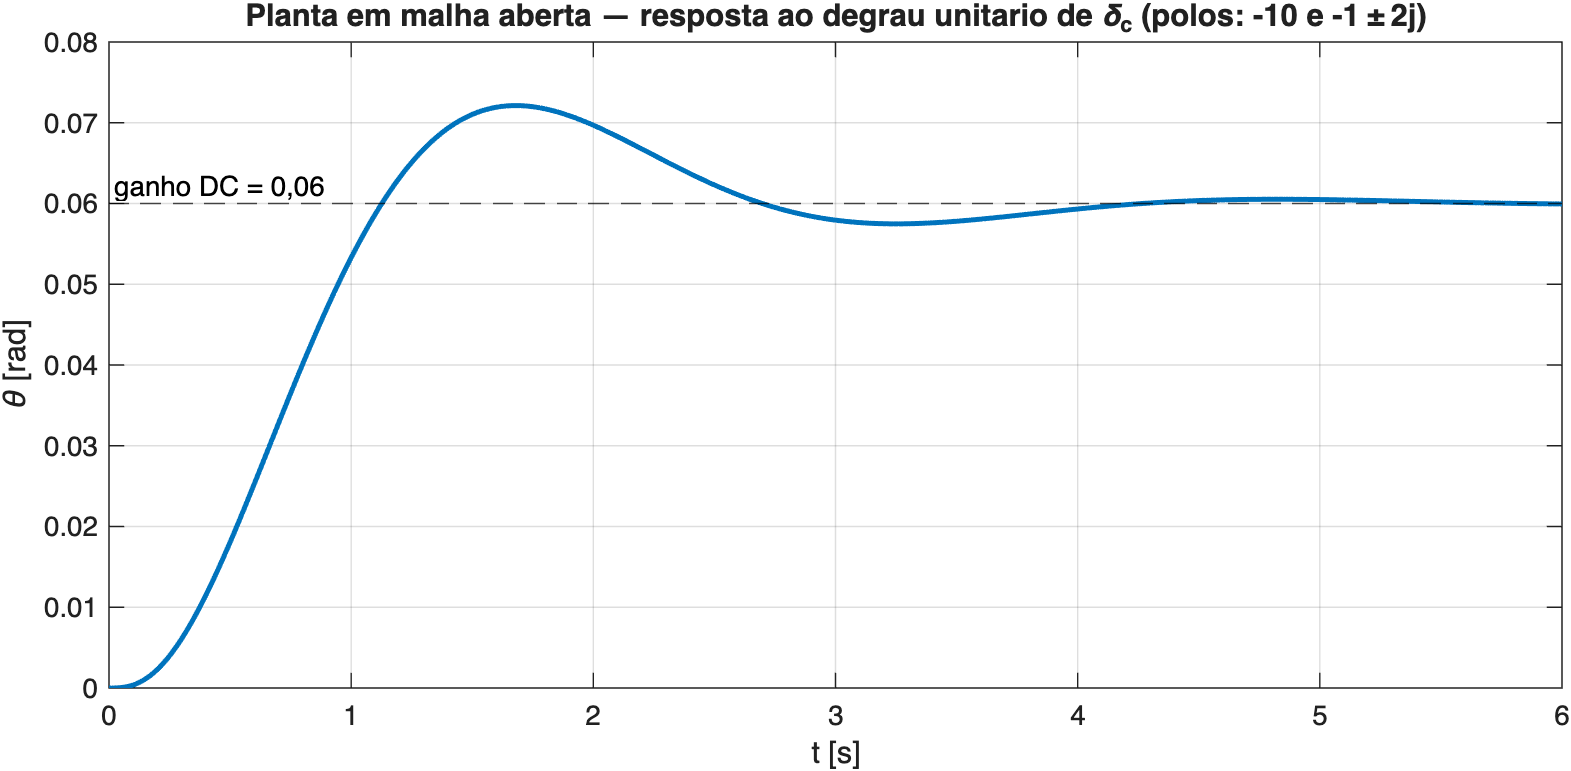
\includegraphics[width=0.82\textwidth]{planta_malha_aberta.png}
  \caption{Planta em \textbf{malha aberta}: resposta de $\theta$ a um degrau
  \emph{unitário} no comando do elevador ($\delta_c=1$). A saída oscila (polos
  $-1\pm2j$, $\zeta\approx0{,}45$) e se acomoda em $0{,}06$ (o ganho DC), proporcional à
  entrada. Em malha aberta não há referência nem realimentação: a planta sozinha não
  leva $\theta$ a um valor desejado.}
  \label{fig:aberta}
\end{figure}

\subsection{O controlador PI de referência}

O controlador clássico (o ``professor'') é um \textbf{PI} (Proporcional + Integral).
A cada instante ele calcula o comando a partir do erro $e=\thetaref-\theta$:
\begin{equation}
  \delta_c(t)=\underbrace{K_p\,e(t)}_{\text{proporcional}}
             +\underbrace{K_i\!\int_0^t e(\tau)\,d\tau}_{\text{integral}}.
  \label{eq:pi}
\end{equation}
A ação integral confere à malha tipo~1, garantindo erro de regime nulo a referências em
degrau. Vale fixar esta parcela: é a integral --- dependente de \emph{todo} o histórico
de $e$ --- que a rede precisará reproduzir a partir apenas de $e(t)$, e que se mostrará o
ponto frágil fora do envelope de treino.

Optou-se por PI (sem o termo derivativo $K_d$) porque (i)~a planta já é adequadamente
amortecida ($\zeta\approx0{,}45$), dispensando o amortecimento da derivada, e (ii)~$K_d$
introduziria ganho de alta frequência, sensível a ruído e difícil de imitar a partir
somente de $e(t)$.

Sintonia via \texttt{pidtune} sobre $G_p$: $K_p=11{,}79$, $K_i=15{,}15$. A malha fechada
resultante apresenta sobressinal $\approx1{,}3\%$, $t_s(2\%)\approx5{,}6$~s,
$t_r\approx0{,}82$~s e erro de regime nulo. Implementação discreta a $T_s=0{,}01$~s
(100~Hz), com a planta contínua integrada por \texttt{ode4} (passo fixo) e o PI
discretizado por \emph{Forward Euler} (bloco PID do Simulink).

\begin{figure}[H]
  \centering
  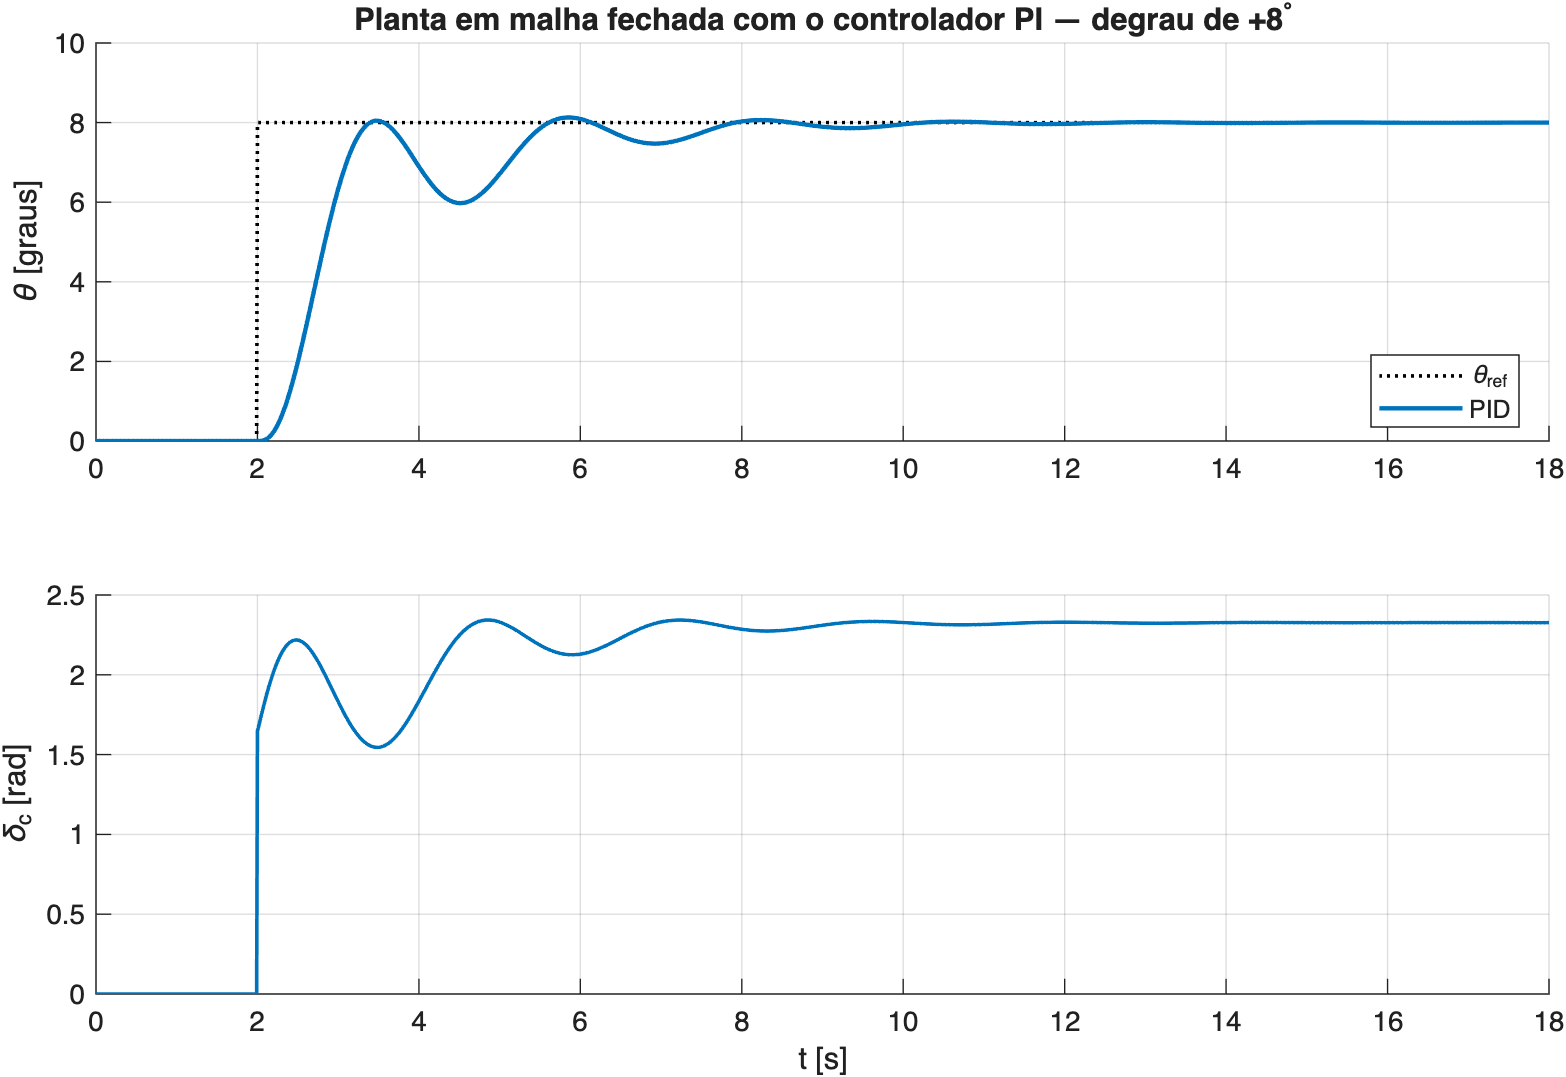
\includegraphics[width=0.82\textwidth]{malha_fechada_pi.png}
  \caption{A planta em \textbf{malha fechada} com o PI, para um degrau de $+8^\circ$.
  Ao contrário da malha aberta (Fig.~\ref{fig:aberta}), agora a saída $\theta$
  \emph{rastreia} a referência: sobressinal pequeno ($\approx1{,}3\%$), acomodação em
  $\approx5{,}6$~s e \textbf{erro de regime nulo} --- graças à ação integral.
  \textbf{Abaixo:} o comando $\delta_c$ que o controlador envia à planta.}
  \label{fig:malhafechada}
\end{figure}

\subsection{A implementação no Simulink}
\label{sec:simulink}

A malha foi montada no Simulink (Fig.~\ref{fig:slx-pid}) --- é a tradução direta do
diagrama da Fig.~\ref{fig:malha}. O bloco \texttt{theta\_ref\_src} gera a referência
$\thetaref$; \texttt{sum\_e} forma o erro $e=\thetaref-\theta$; o bloco
\textbf{Controlador} (aqui o PI discreto, \texttt{PI(z)}) produz o comando $\delta_c$; e
a planta é fechada por $G_{\mathrm{elev}}$ (função de transferência $Y/U$) seguida de
$G_{\mathrm{din}}$ (implementada em \textbf{espaço de estados}
$\dot x=Ax+Bu,\;y=Cx+Du$, justamente para expor a condição inicial $\theta(0)$ usada nos
testes de robustez). A saída $\theta$ realimenta o somador, e os blocos \texttt{out.*}
apenas registram os sinais ($\thetaref$, $e$, $\delta_c$, $\theta$) para análise
posterior.

O ponto central do trabalho aparece aqui de forma literal: os modelos
\texttt{pitch\_PID.slx} e \texttt{pitch\_LSTM.slx} são \emph{idênticos}, exceto pelo
bloco \textbf{Controlador} --- é exatamente o ``bloco substituído'' da
Fig.~\ref{fig:malha}. Nesta seção ele é o \texttt{PI(z)}; ao trocá-lo pela rede obtém-se
o modelo da Fig.~\ref{fig:slx-malha} (Seção~\ref{sec:treino-como}), cujo interior está
detalhado na Fig.~\ref{fig:slx-ctrl}.

\begin{figure}[H]
  \centering
  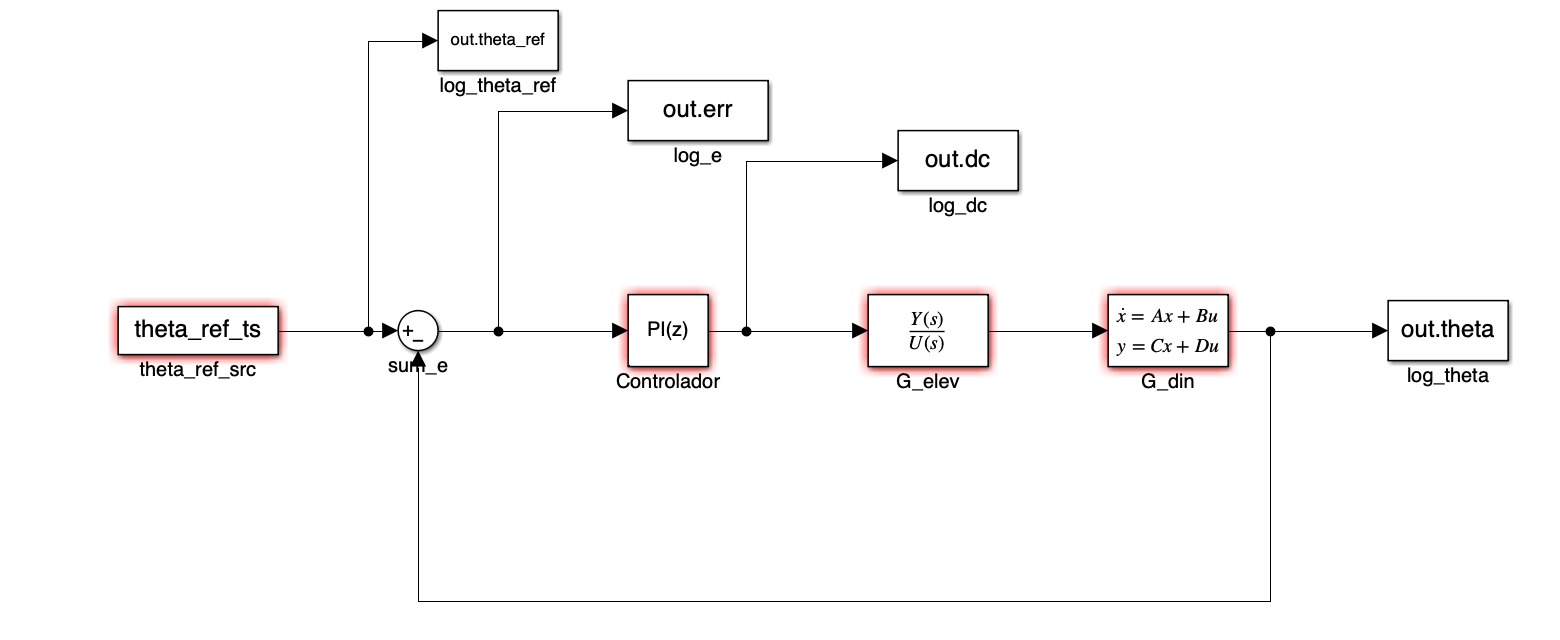
\includegraphics[width=\textwidth]{simulink_malha_pid.png}
  \caption{A malha de controle no \textbf{Simulink} (modelo \texttt{pitch\_PID.slx}),
  realização concreta do diagrama da Fig.~\ref{fig:malha}. Da esquerda para a direita:
  a referência $\thetaref$, o somador que forma o erro $e$, o \textbf{Controlador}
  (aqui o bloco \texttt{PI(z)}), o servo $G_{\mathrm{elev}}$ e a dinâmica
  $G_{\mathrm{din}}$ em espaço de estados, com a saída $\theta$ realimentando a entrada.
  Os blocos à parte (\texttt{out.theta\_ref}, \texttt{out.err}, \texttt{out.dc},
  \texttt{out.theta}) só registram os sinais para análise.}
  \label{fig:slx-pid}
\end{figure}

% =====================================================================
\section{O que é uma rede neural LSTM?}
\label{sec:lstm}
% =====================================================================

Esta seção apresenta a rede neural utilizada. A exposição apoia-se em analogias com
sistemas dinâmicos --- a principal delas sendo que \textbf{uma LSTM é, em essência, um
sistema dinâmico discreto com estado, cujas equações são aprendidas a partir de dados}
em vez de deduzidas da física.

\subsection{De um neurônio a uma rede}

A unidade básica é o \textbf{neurônio artificial}: ele recebe alguns números de
entrada, multiplica cada um por um \textbf{peso}, soma tudo (com um termo constante, o
\emph{viés}) e passa o resultado por uma função simples e não linear (uma ``curva em S'',
por exemplo). Uma \textbf{rede neural} é apenas muitos desses neurônios organizados em
\textbf{camadas}, onde a saída de uma camada alimenta a próxima. Toda a ``inteligência''
está nos \emph{pesos} --- e \textbf{treinar} a rede significa, simplesmente, ajustar
esses pesos até que a saída dela fique o mais próxima possível da saída desejada (aqui,
o comando que o PID daria). É um problema de \emph{regressão}, como ajustar uma curva a
pontos, só que com muitos parâmetros.

\subsection{O ingrediente que falta numa rede comum: memória}

Uma rede neural comum (dita \emph{feedforward}) comporta-se como um \textbf{ganho
estático não linear}: para a mesma entrada, devolve sempre a mesma saída, sem nenhuma
noção de passado. Isso é fatal para o nosso problema, porque o comando do PID
\textbf{não} depende só do erro atual --- o termo integral $K_i\!\int e$ depende de
\emph{todo} o histórico do erro. Uma rede sem memória não teria como reproduzir essa
parcela.

A \textbf{LSTM} (\emph{Long Short-Term Memory}, ``memória de curto-longo prazo'')
resolve isso carregando um \textbf{estado interno} que ela atualiza a cada instante.
Em linguagem de controle, isso é \emph{exatamente} um sistema dinâmico discreto:
\begin{equation}
  h[k] = f\big(h[k-1],\, e[k]\big), \qquad
  \delta_c[k] = g\big(h[k]\big),
  \label{eq:lstm-ss}
\end{equation}
onde o vetor $h$ é o \textbf{estado} (a ``memória'') da rede --- o análogo direto do
vetor de estados $x$ de uma representação em espaço de estados, ou do acumulador do
integrador do PID. A diferença para um modelo clássico é que as funções $f$ e $g$ não
são escritas à mão a partir da física: elas são \textbf{aprendidas dos dados}. É essa
memória, governada por~\eqref{eq:lstm-ss}, que permite à rede representar a ação
integral acumulada ao longo de um episódio.

\subsection{As ``comportas'' que dão nome à LSTM}

O que distingue a LSTM de outras redes com memória é \emph{como} ela decide o que
guardar e o que descartar. Cada unidade possui três \textbf{comportas} (\emph{gates}) ---
pequenas válvulas com abertura contínua entre 0 (fechada) e 1 (aberta), cujos ajustes
também são aprendidos:
\begin{itemize}
  \item a \textbf{comporta de esquecimento} decide quanto do estado anterior manter;
  \item a \textbf{comporta de entrada} decide quanto da informação nova incorporar;
  \item a \textbf{comporta de saída} decide quanto do estado interno expor na saída.
\end{itemize}
Na prática, essas comportas permitem que a rede preserve uma informação relevante por
centenas ou milhares de passos sem que ela ``vaze'' --- comportamento ideal para
representar um acumulador, como a integral do erro. É daí que vem o nome: memória que
pode ser tanto de \emph{curto} quanto de \emph{longo} prazo, conforme a tarefa exigir.

\subsection{A arquitetura usada neste trabalho}

A rede recebe \emph{um} número por instante (o erro $e[k]$) e devolve \emph{um} número
(o comando $\delta_c[k]$). Entre a entrada e a saída há duas camadas LSTM empilhadas, com
64 e 32 unidades, seguidas de uma camada \emph{totalmente conectada} que combina
linearmente o resultado num único valor (Fig.~\ref{fig:arq}).

\begin{figure}[H]
\centering
\begin{tikzpicture}[>=Latex, font=\small, node distance=10mm,
  io/.style={draw, rounded corners=2pt, minimum height=11mm, minimum width=15mm, align=center, fill=gray!10},
  lstm/.style={draw, rounded corners=2pt, minimum height=11mm, minimum width=22mm, align=center, fill=orange!18},
  fc/.style={draw, rounded corners=2pt, minimum height=11mm, minimum width=20mm, align=center, fill=blue!10}]
  \node[io] (in) {entrada\\$e[k]$};
  \node[lstm, right=of in] (l1) {LSTM\\64 unid.};
  \node[lstm, right=of l1] (l2) {LSTM\\32 unid.};
  \node[fc, right=of l2] (fc) {camada\\linear};
  \node[io, right=of fc] (out) {saída\\$\delta_c[k]$};
  \draw[->] (in) -- (l1);
  \draw[->] (l1) -- (l2);
  \draw[->] (l2) -- (fc);
  \draw[->] (fc) -- (out);
  % laco de estado (memoria)
  \draw[->, orange!70!black, thick] (l1.north) ++(0,1mm) .. controls +(0,6mm) and +(0,6mm) .. ($(l1.north)+(-0.1mm,1mm)$);
  \node[orange!70!black, font=\footnotesize, above=5.5mm of l1] {estado $h$ (memória)};
\end{tikzpicture}
\caption{Arquitetura da rede: um erro entra por instante, passa por duas camadas LSTM
(que carregam o estado/memória $h$) e por uma camada linear, e sai um comando. É a
versão ``aprendida'' do controlador --- compare com a Eq.~\eqref{eq:lstm-ss}.}
\label{fig:arq}
\end{figure}

Por que \emph{duas} camadas e justamente esses tamanhos? Em testes preliminares, camadas
menores (32 e 16 unidades) não conseguiam manter o acumulador integral com precisão por
milhares de passos: a resposta à \emph{rampa} (dominada pela parcela $K_i\!\int e$)
ficava pobre. Com $64\to32$ a rede ganha ``espaço'' suficiente para representar bem a
ação integral, sem ficar grande a ponto de decorar os dados.

\subsection{Como a rede é treinada}
\label{sec:treino-como}

Treinar é resolver um problema de otimização: ajustar os pesos para minimizar o
\textbf{erro quadrático médio} (MSE) entre o comando que a rede produz e o comando que o
PID produziu, somado sobre todos os exemplos. Os principais elementos do treino:
\begin{itemize}
  \item \textbf{Normalização.} Antes de entrar na rede, o erro é reescalado para ter
        média~0 e desvio~1 (\emph{z-score}); a saída é ``desnormalizada'' de volta para
        graus de comando. Isso só deixa os números numa escala confortável para o
        treino --- na malha de controle, aparece como pequenos blocos de ganho e viés em
        torno da LSTM.
  \item \textbf{Otimizador.} Usamos o algoritmo \emph{Adam}, com até 350 \emph{épocas}
        (passagens pelos dados) e taxa de aprendizado inicial $3\times10^{-3}$, reduzida
        pela metade periodicamente para refinar o ajuste no fim.
  \item \textbf{Validação e parada antecipada.} Separamos os episódios em 70\,\% para
        treino, 15\,\% para validação e 15\,\% para teste. Guardamos a versão da rede com
        \emph{melhor} desempenho na validação (\emph{early stopping}): isso evita a
        ``decoreba'' (\emph{overfitting}), em que a rede memoriza os exemplos mas vai mal
        em casos novos.
  \item \textbf{Episódio inteiro.} Treinamos com a sequência completa de cada manobra
        (não com janelas curtas), para que o estado da LSTM acumule a integral desde
        $t=0$ --- exatamente como ela opera depois na malha fechada.
\end{itemize}

Na malha de controle, a rede treinada substitui o bloco \texttt{PI(z)} por um subsistema
\textbf{Controlador}: o modelo \texttt{pitch\_LSTM.slx} (Fig.~\ref{fig:slx-malha}) é
\emph{idêntico} ao \texttt{pitch\_PID.slx} (Fig.~\ref{fig:slx-pid}), trocando apenas esse
bloco. Por dentro (Fig.~\ref{fig:slx-ctrl}), o subsistema é a arquitetura da
Fig.~\ref{fig:arq} embrulhada pela normalização descrita acima: o erro $e$ entra, é
normalizado, atravessa a rede recorrente operando em modo \emph{Stateful Predict} (que
mantém o estado/memória $h$ entre os passos da simulação) e é desnormalizado de volta
para o comando $\delta_c$ em graus.

\begin{figure}[H]
  \centering
  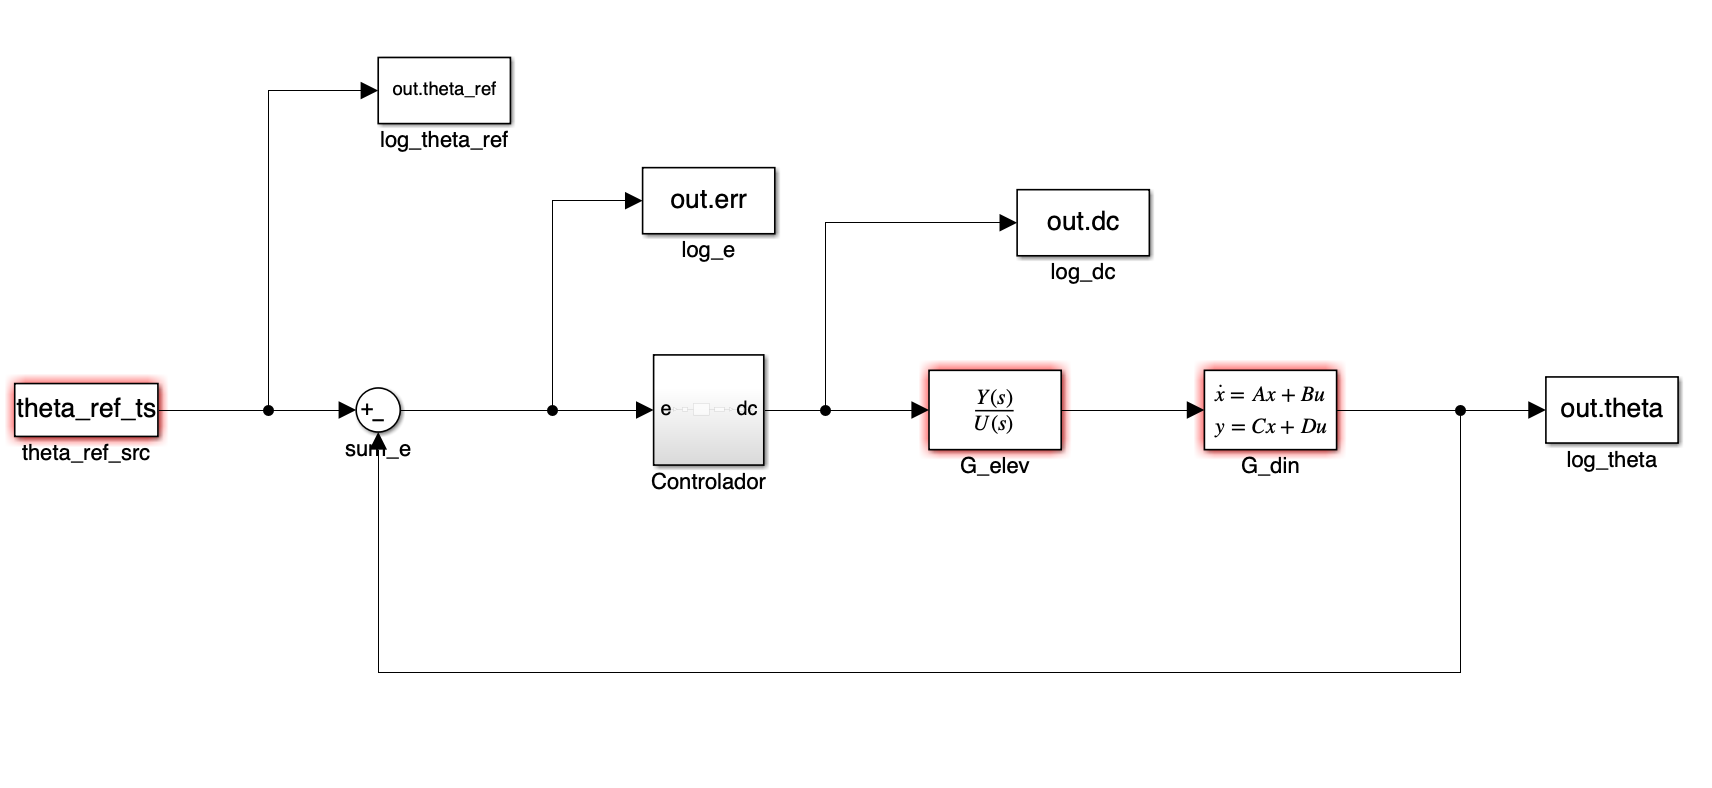
\includegraphics[width=\textwidth]{simulink_malha.png}
  \caption{A mesma malha da Fig.~\ref{fig:slx-pid}, agora no modelo
  \texttt{pitch\_LSTM.slx}: tudo é igual ao caso do PID, exceto o bloco
  \textbf{Controlador}, que deixou de ser o \texttt{PI(z)} e passou a ser o subsistema da
  rede neural (detalhado na Fig.~\ref{fig:slx-ctrl}). É a materialização do ``bloco
  substituído'' da Fig.~\ref{fig:malha}.}
  \label{fig:slx-malha}
\end{figure}

\begin{figure}[H]
  \centering
  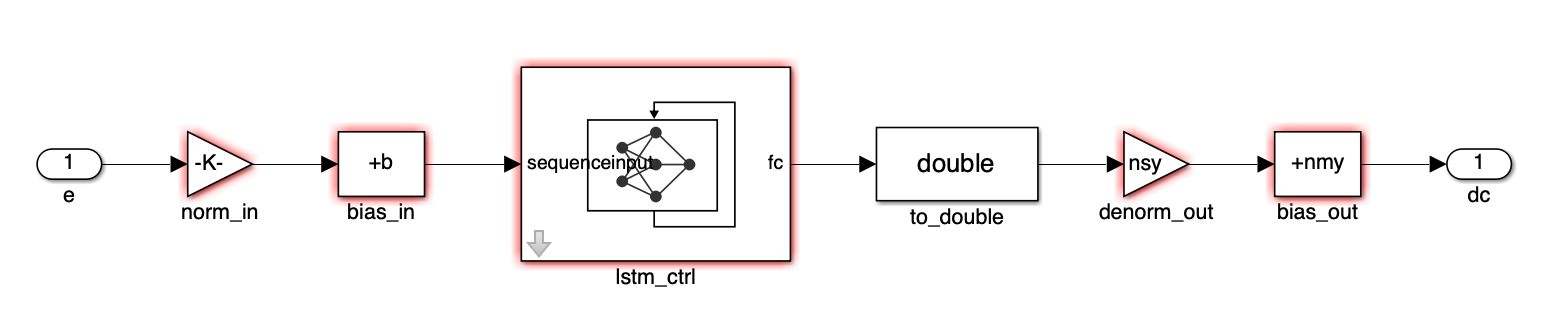
\includegraphics[width=\textwidth]{simulink_controlador_lstm.png}
  \caption{O subsistema \textbf{Controlador} do \texttt{pitch\_LSTM.slx} por dentro ---
  o ``bloco substituído'' da Fig.~\ref{fig:malha}. O erro $e$ é normalizado
  (\texttt{norm\_in}: ganho $-K-$ e viés $+b$, o \emph{z-score}), passa pela rede
  recorrente (\texttt{lstm\_ctrl}: \texttt{sequenceinput}$\to$LSTM$\to$\texttt{fc}) em
  \emph{Stateful Predict}, é convertido para \texttt{double} e desnormalizado
  (\texttt{denorm\_out}/\texttt{bias\_out}) de volta para o comando $\delta_c$. É a
  Eq.~\eqref{eq:lstm-ss}/Fig.~\ref{fig:arq} com a (des)normalização ao redor.}
  \label{fig:slx-ctrl}
\end{figure}

A próxima seção descreve o procedimento de treinamento da rede para controlar o avião.

% =====================================================================
\section{Como a rede neural aprende}
% =====================================================================

\subsection{Aprender por imitação}

A estratégia é simples de explicar: deixamos o controlador clássico comandar o avião
em milhares de situações simuladas e \textbf{anotamos tudo} --- em cada instante, qual
era o erro e qual foi o comando dado. Isso vira uma grande tabela de exemplos
``situação $\to$ comando''. A rede neural então treina para \textbf{reproduzir} esses
exemplos: dado o histórico do erro, ela tenta dar o mesmo comando que o professor
daria. É o que se chama \emph{aprender por imitação}.

Usamos uma rede do tipo \textbf{LSTM}~\cite{hochreiter1997}, descrita na
Seção~\ref{sec:lstm}: a característica que importa aqui é que ela tem \textbf{memória}
(o estado interno $h$) --- lembra do que aconteceu nos instantes anteriores. Isso é
essencial porque o professor também tem memória (aquela parcela do ``acúmulo do erro'',
a integral). Sem memória, a rede não conseguiria imitá-lo.

\subsection{Por que só imitar não basta: o DAgger}
\label{sec:dagger}

Aqui está o ponto mais importante do trabalho, e vale uma analogia:

\begin{quote}
Imagine ensinar alguém a dirigir mostrando \emph{só} vídeos de um motorista experiente
numa estrada perfeita. A pessoa decora aquilo. Mas, quando assume o volante e comete um
pequeno desvio, ela se vê numa situação que \textbf{nunca apareceu nos vídeos} --- e não
sabe como reagir. O pequeno erro vira um erro maior, e ela perde o controle.
\end{quote}

Foi exatamente o que aconteceu com a rede de imitação pura. No papel ela ia muito bem
(copiava o comando do PID com fidelidade alta). Mas, ao assumir o comando do avião,
qualquer errinho a levava a uma situação que o PID nunca havia criado --- e ali ela não
sabia o que fazer. O resultado é a curva vermelha da Figura~\ref{fig:dagger}: a rede
entra em \textbf{oscilação} (um ``ciclo-limite''), balançando o nariz do avião sem parar,
enquanto o PID rastreia limpo.

\begin{figure}[H]
  \centering
  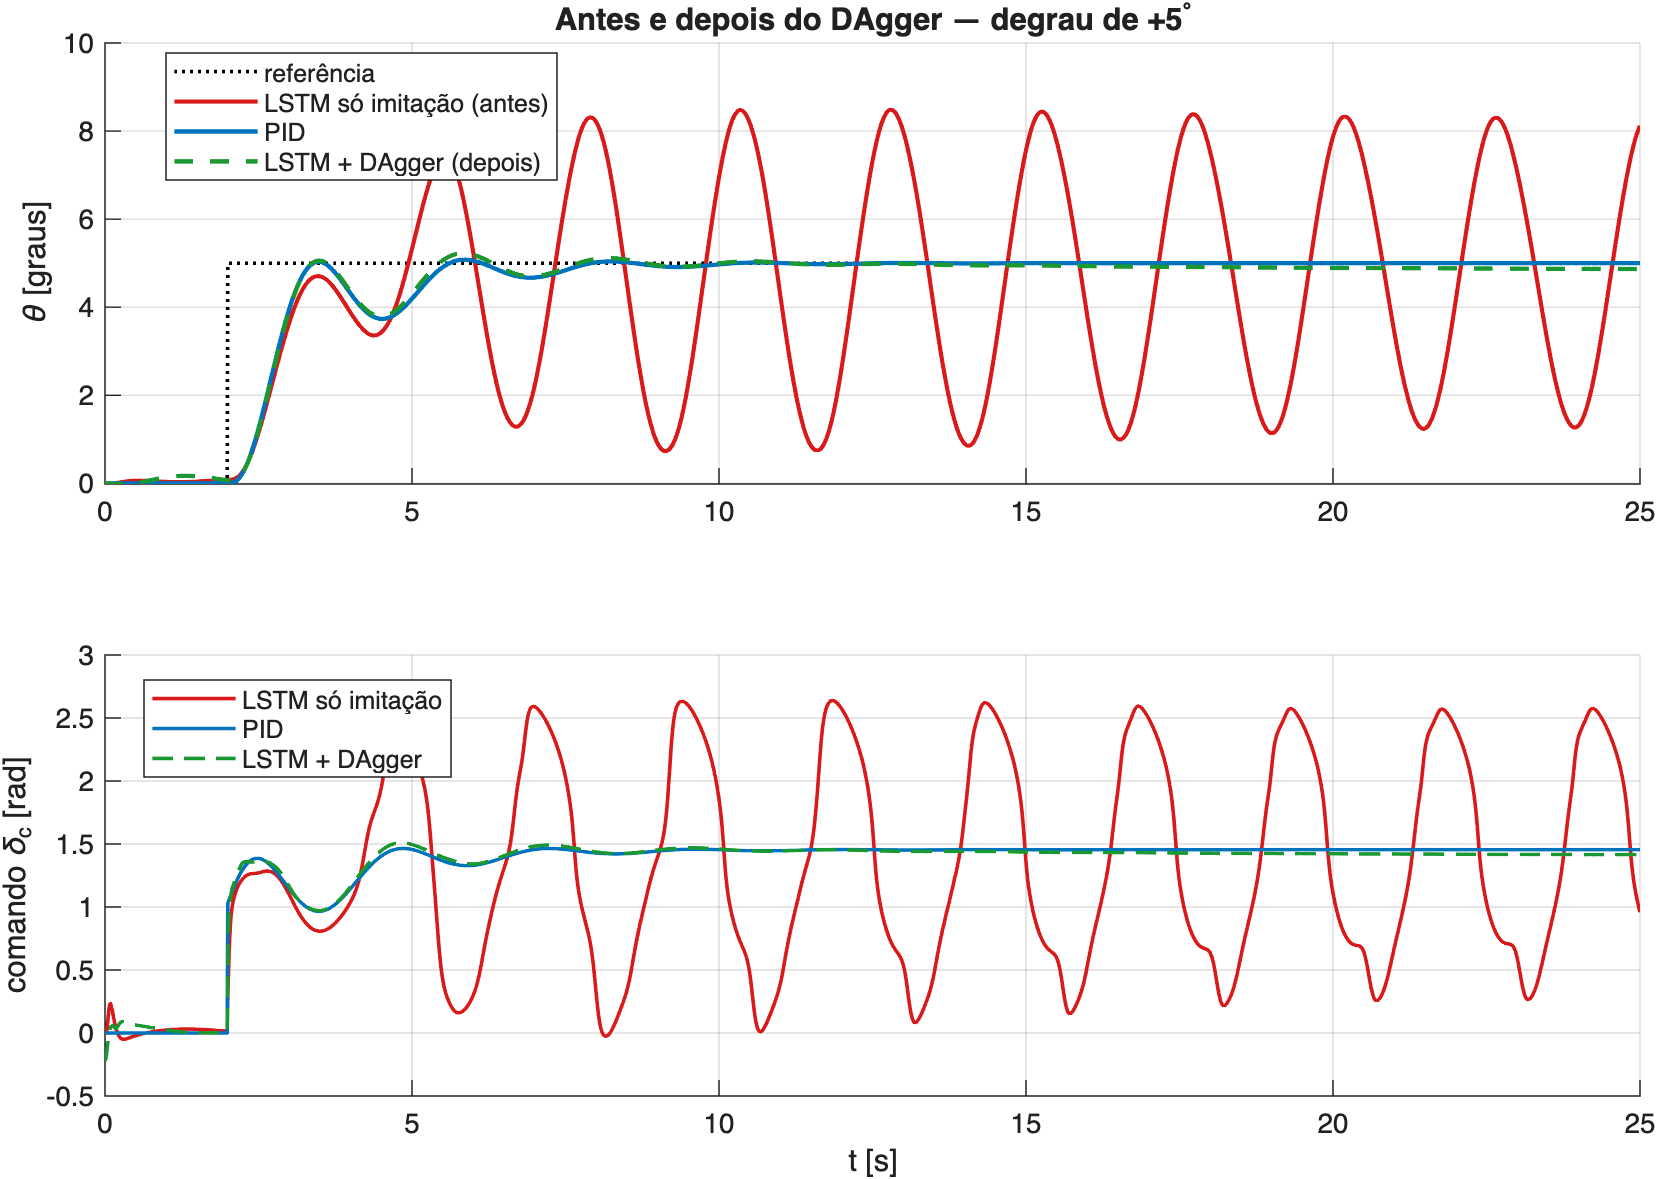
\includegraphics[width=0.86\textwidth]{dagger_antes_depois.png}
  \caption{O efeito do DAgger, num degrau de $+5^\circ$. \textbf{Vermelho:} a rede de
  imitação pura oscila sem parar em malha fechada. \textbf{Azul:} o PID.
  \textbf{Verde tracejado:} a \emph{mesma} rede após o DAgger --- a oscilação desaparece
  e ela passa a acompanhar o PID.}
  \label{fig:dagger}
\end{figure}

A causa tem nome técnico: \emph{desvio de distribuição} (em inglês, \emph{distribution
shift}). A imitação simples treina a rede \emph{apenas} nas situações que o professor
(o PID) percorre; mas, no comando, a rede gera situações \emph{próprias} --- justamente
as que os erros dela criam --- e nessas ela nunca foi treinada. Como nunca aprendeu a
corrigi-las, os erros se acumulam até virar a oscilação.

O \textbf{DAgger} (do inglês \emph{Dataset Aggregation}, ``agregação de dados''; Ross
\emph{et al.}~\cite{ross2011}) é um método \emph{iterativo} que ataca exatamente isso.
A cada rodada:
\begin{enumerate}
  \item a rede \emph{atual} comanda o avião, e nós registramos as situações (os erros
        $e(t)$) que \textbf{ela mesma} visita --- inclusive as oscilatórias;
  \item para cada uma dessas situações, perguntamos ao professor ``o que você faria
        aqui?'' e guardamos a resposta certa (o comando do PID);
  \item \textbf{agregamos} esses novos exemplos ao banco --- sem descartar os antigos,
        daí o nome ``agregação'' --- e \textbf{treinamos de novo}.
\end{enumerate}
A cada repetição, o banco passa a conter cada vez mais as situações que a rede
\emph{de fato} encontra, e ela aprende a se recuperar dos próprios erros. Um detalhe que
torna o método viável aqui: o professor precisa saber responder em \emph{qualquer}
situação --- e o PID, por ser uma fórmula ($\delta_c=K_p\,e+K_i\!\int e$), pode ser
consultado em qualquer erro, sem custo. Fizemos \textbf{duas rodadas}; ao fim, a
oscilação havia desaparecido (a curva verde da Fig.~\ref{fig:dagger}).

Para tornar o laço concreto, vale segui-lo no próprio caso do degrau de $+5^\circ$
(Fig.~\ref{fig:dagger}).

\paragraph{Passo 1 --- o que se grava.} Rodamos a malha fechada com a rede \emph{atual}
(a que oscila) no comando. A cada passo de tempo (100~Hz, $\approx2500$ pontos no
episódio) gravamos \textbf{o erro que a malha visitou},
\[
  e(t)=\thetaref(t)-\theta(t).
\]
Como a rede oscila, esse $e(t)$ também oscila --- é o ``espelho'' da curva vermelha:
quando a rede deixa $\theta$ subir a $8{,}5^\circ$, o erro vai a $5-8{,}5=-3{,}5^\circ$;
quando $\theta$ cai a $1{,}5^\circ$, o erro vai a $+3{,}5^\circ$. Guardamos \emph{o erro}
(a ``situação''), que será a \textbf{entrada} do retreino; \emph{não} guardamos o
comando que a rede deu --- esse é o comportamento ruim, que não queremos copiar. Só
precisamos saber em \emph{quais situações} ela se meteu.

\paragraph{Passo 2 --- ``o que você faria aqui?''.} O professor é o PID, que é apenas a
fórmula $\delta_c=K_p e+K_i\!\int e$. Então, para rotular cada situação, não
re-simulamos nada: \textbf{aplicamos a fórmula do PID ao erro gravado}, instante a
instante --- com a mesma integração discreta do integrador do PID:
\[
  I[k]=I[k-1]+T_s\,e[k-1], \qquad
  \delta_c^{\mathrm{PID}}[k]=K_p\,e[k]+K_i\,I[k].
\]
Ou seja, para \emph{cada} instante da oscilação obtemos o comando correto. No exemplo:
naquele momento em que $\theta$ havia passado para $8{,}5^\circ$ (erro $-3{,}5^\circ$),
o rótulo do PID manda o comando \emph{para baixo}, para derrubar o nariz --- exatamente
a ação corretiva que a rede oscilante não soube fazer. O novo exemplo de treino é o par
de sequências $\;\underbrace{e(t)}_{\text{entrada (erro visitado)}}\longrightarrow
\underbrace{\delta_c^{\mathrm{PID}}(t)}_{\text{alvo (comando certo)}}$.

\paragraph{Passo 3 --- como entra no retreino.} Esse par é \textbf{somado} ao banco
original (os 240 episódios do PID) --- agregação, não substituição --- e a rede retreina
no conjunto inteiro, com a mesma formulação sequência-a-sequência. A diferença é
decisiva: \emph{antes}, o banco só tinha trajetórias suaves do PID (que nunca oscila), e
a rede nunca via ``$\theta$ passou do ponto e está oscilando $\to$ comando corretivo'';
\emph{depois}, o banco contém justamente essas situações oscilatórias rotuladas com a
resposta amortecedora do PID. Ao reencontrar esses estados em operação, a rede agora
sabe o que fazer --- e a oscilação some.

Vale destacar que essa combinação --- uma \textbf{rede LSTM treinada por imitação e
refinada com DAgger} para substituir um controlador clássico --- não é exclusiva deste
trabalho. Espin \emph{et al.}~\cite{espin2024}, por exemplo, usaram exatamente essa
estratégia (rede recorrente LSTM + \emph{behavior cloning} + DAgger) para emular um
controlador preditivo (MPC) no carregamento ótimo de baterias, com a mesma motivação
que a nossa: a imitação pura sofre de desvio de distribuição, e o DAgger o corrige
realimentando os estados que a própria rede visita. O uso de redes recorrentes em
aprendizado por imitação também é estudado de forma mais geral em~\cite{nguyen2016}.

% =====================================================================
\section{Os dados de treinamento}
% =====================================================================

A rede aprende por imitação, então tudo depende dos exemplos que mostramos a ela. Esta
seção descreve \emph{quais} dados foram usados e \emph{como} foram gerados.

\subsection{A ideia: o PID gera os dados}

Não programamos a rede com regras. Em vez disso, deixamos o controlador PID comandar a
planta em simulação e gravamos, a cada instante, um par
\[
  \underbrace{e(t)=\thetaref-\theta}_{\text{entrada}}
  \qquad\longrightarrow\qquad
  \underbrace{\delta_c(t)\ \text{(comando do PID)}}_{\text{alvo}} .
\]
Esses pares ``erro $\to$ comando'' são os exemplos de treino: a rede deve, a partir do
histórico do erro, produzir o mesmo comando que o PID produziu. A
Figura~\ref{fig:par} mostra um episódio: o PID controla a planta (acima), e dele
extraímos a entrada $e(t)$ (meio) e o alvo $\delta_c(t)$ (abaixo), amostrados a 100~Hz.

\begin{figure}[H]
  \centering
  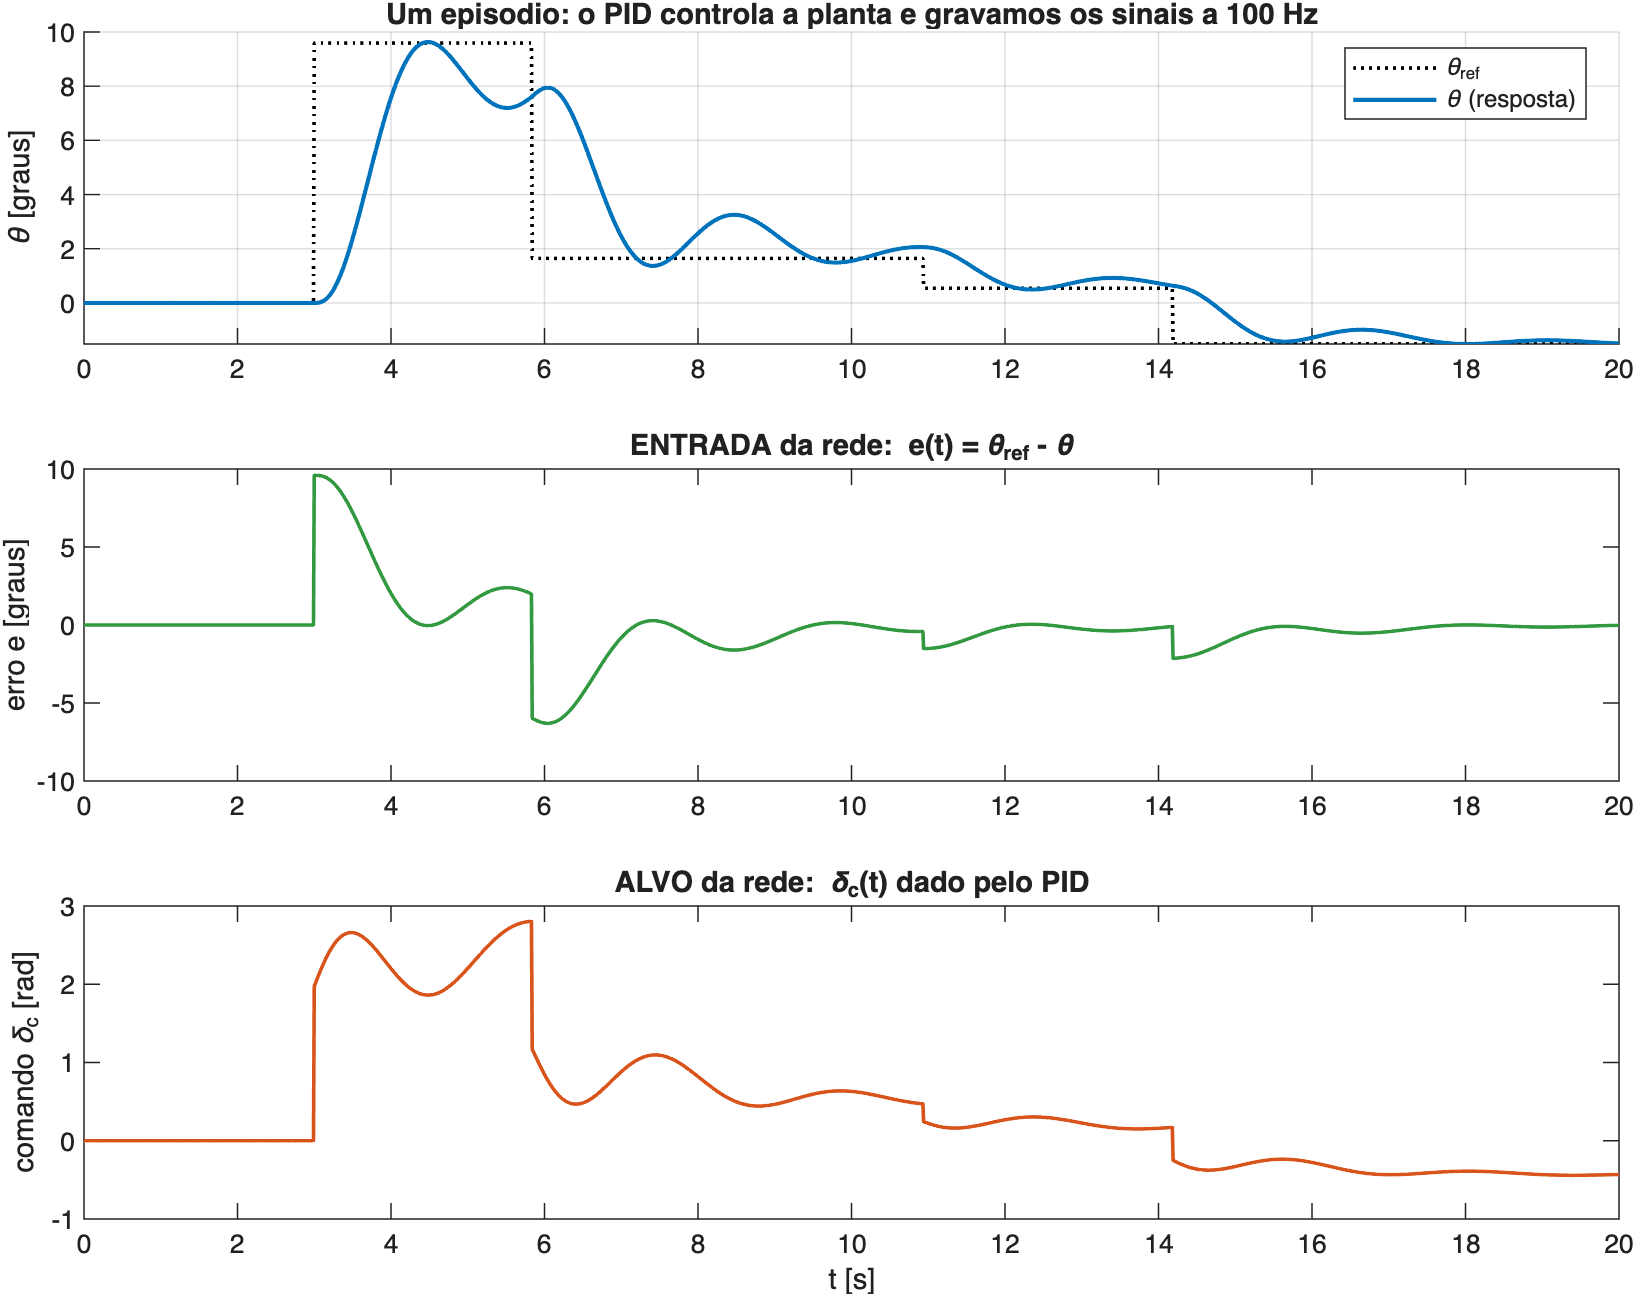
\includegraphics[width=0.80\textwidth]{dados_par.png}
  \caption{De cada simulação extraímos os sinais que treinam a rede. \textbf{Acima:} o
  PID segue a referência $\thetaref$. \textbf{Meio:} a \emph{entrada} da rede, o erro
  $e=\thetaref-\theta$. \textbf{Abaixo:} o \emph{alvo}, o comando $\delta_c$ que o PID
  enviou. A rede aprende o mapa $e(t)\to\delta_c(t)$.}
  \label{fig:par}
\end{figure}

\subsection{Variedade: cobrindo muitas situações}

Para generalizar, a rede precisa ver muitas situações diferentes --- não só um degrau.
Por isso rodamos a malha fechada com \textbf{quatro famílias de referência}
$\thetaref(t)$, sorteadas aleatoriamente (Fig.~\ref{fig:perfis}):
\begin{itemize}
  \item \textbf{degraus}: 2 a 4 saltos, em instantes e amplitudes aleatórios;
  \item \textbf{doublet}: um pulso $+A$ seguido de $-A$;
  \item \textbf{rampa}: subida gradual, patamar e descida;
  \item \textbf{multisseno}: soma de 3 a 5 senoides ($0{,}05$--$0{,}5$~Hz).
\end{itemize}
Todas as referências ficam dentro de $\pm10^\circ$, e os episódios começam com a planta
nivelada. Cada episódio dura 20~s a 100~Hz; geramos \textbf{240 episódios} (60 de cada
tipo), totalizando cerca de \textbf{480 mil} pares de treino. Usou-se um \emph{único}
PID: com vários controladores discordantes, a regressão convergiria para uma média sem
significado --- a variedade necessária vem das \emph{manobras}, não do professor.

\begin{figure}[H]
  \centering
  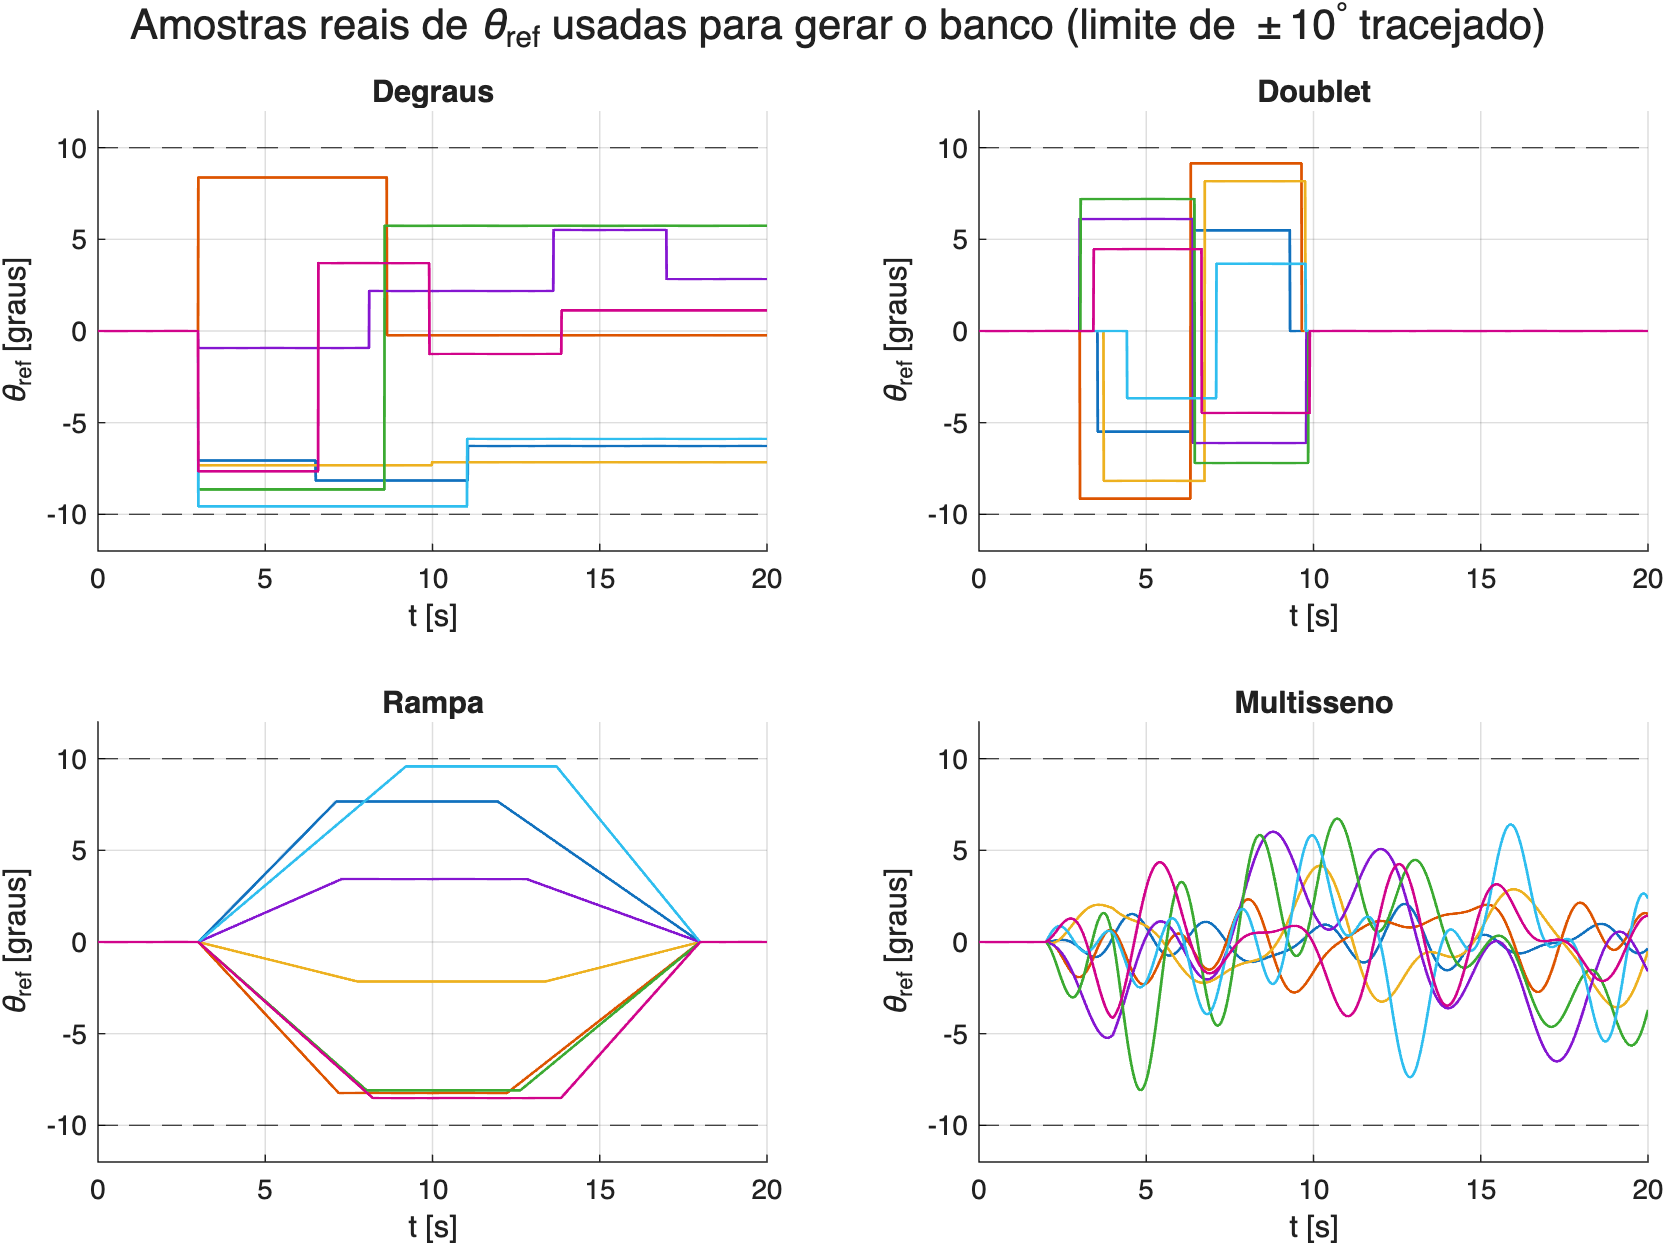
\includegraphics[width=0.92\textwidth]{dados_perfis.png}
  \caption{Amostras reais das quatro famílias de referência $\thetaref$ usadas para
  gerar o banco (sete sorteios de cada, sobrepostos). Todas respeitam o limite de
  $\pm10^\circ$ (linhas tracejadas) --- a faixa de operação que a rede efetivamente
  aprende.}
  \label{fig:perfis}
\end{figure}

\subsection{O reforço do DAgger}

A Seção~\ref{sec:dagger} explicou \emph{por que} o DAgger é necessário (a imitação pura
oscilava em malha fechada, Fig.~\ref{fig:dagger}) e \emph{como} ele funciona. Aqui
registramos apenas \emph{quanto} ele acrescentou ao banco: a própria rede comandou a
planta e, dos erros $e(t)$ que ela visitou (inclusive os estados oscilatórios que o PID
nunca cria), geramos \textbf{136 episódios} extras, cada um rotulado com o comando exato
do PID, $\delta_c=K_p\,e+K_i\!\int e$. Somados aos 240 originais, o banco final tem
\textbf{376 episódios}.

% =====================================================================
\section{Resultado: a rede empata com o controlador clássico}
% =====================================================================

Depois desse treino, colocamos a rede neural para comandar o avião e comparamos com o
controlador clássico nas mesmas situações. As Figuras~\ref{fig:pid} e~\ref{fig:lstm}
mostram um exemplo: pedimos uma inclinação de $+7^\circ$ e depois $-4^\circ$. As duas
curvas (clássico e rede neural) ficam praticamente \textbf{em cima uma da outra}.

\begin{figure}[H]
  \centering
  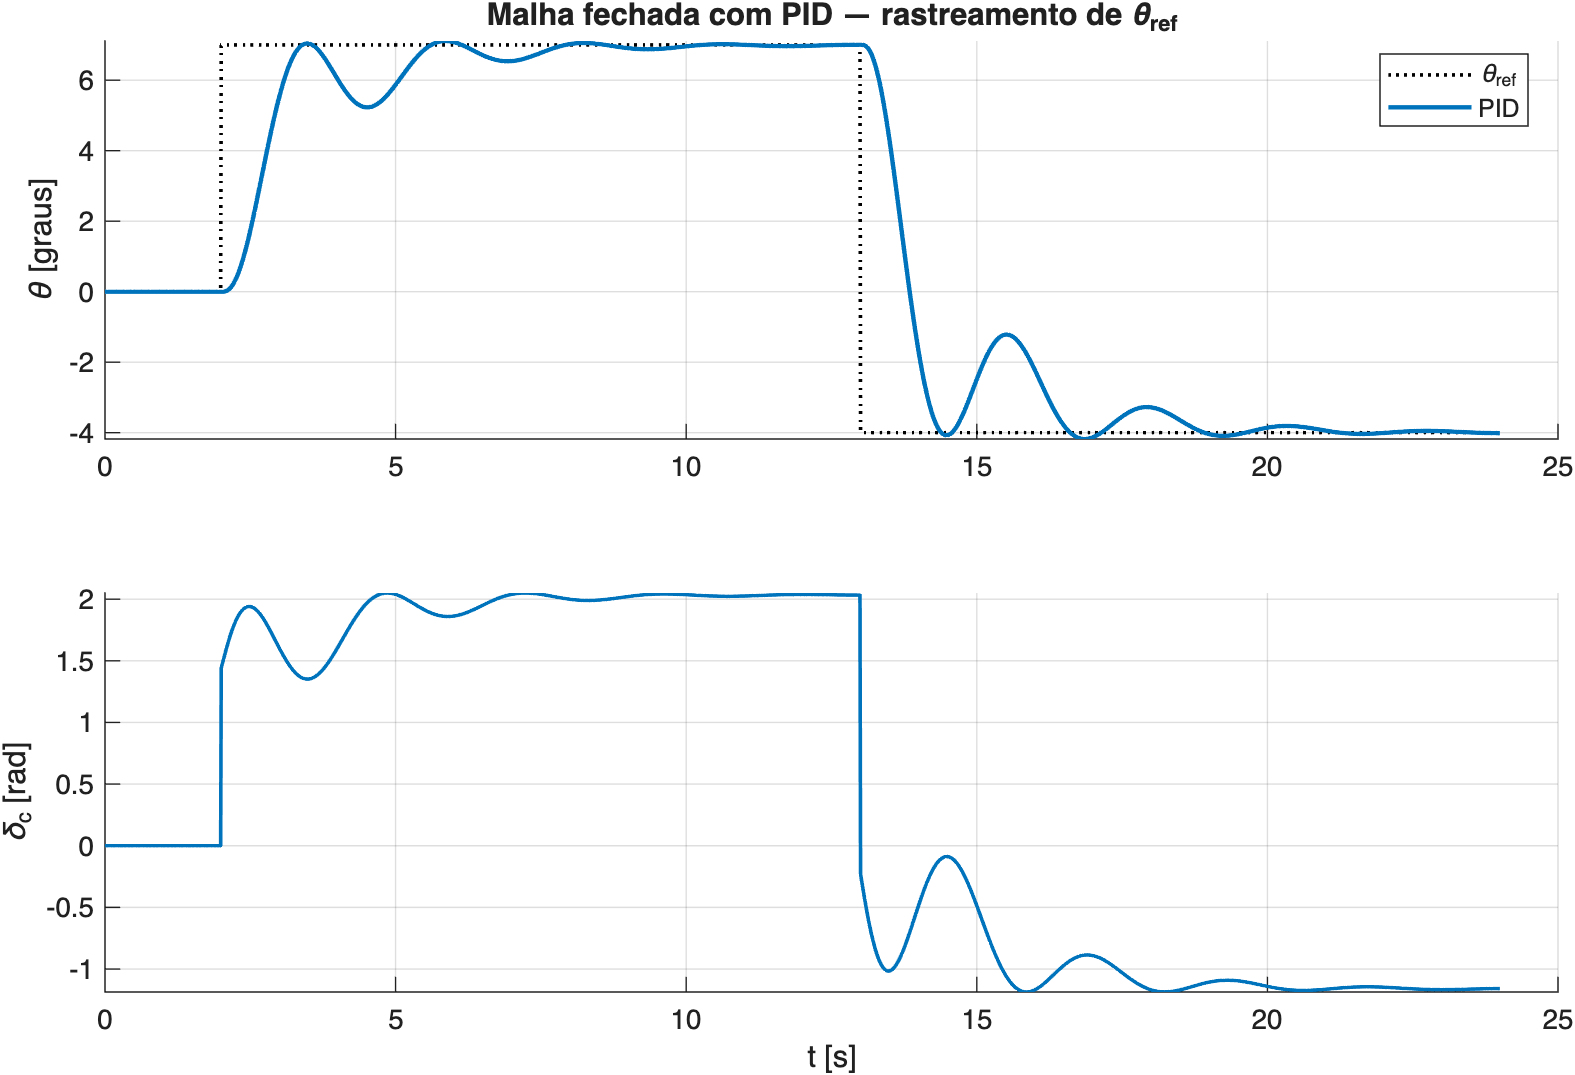
\includegraphics[width=0.84\textwidth]{malha_fechada_pid.png}
  \caption{Avião comandado pelo \textbf{controlador clássico (PID)}. Acima: a
  inclinação (linha cheia) seguindo o alvo (linha pontilhada). Abaixo: o comando
  enviado ao profundor.}
  \label{fig:pid}
\end{figure}

\begin{figure}[H]
  \centering
  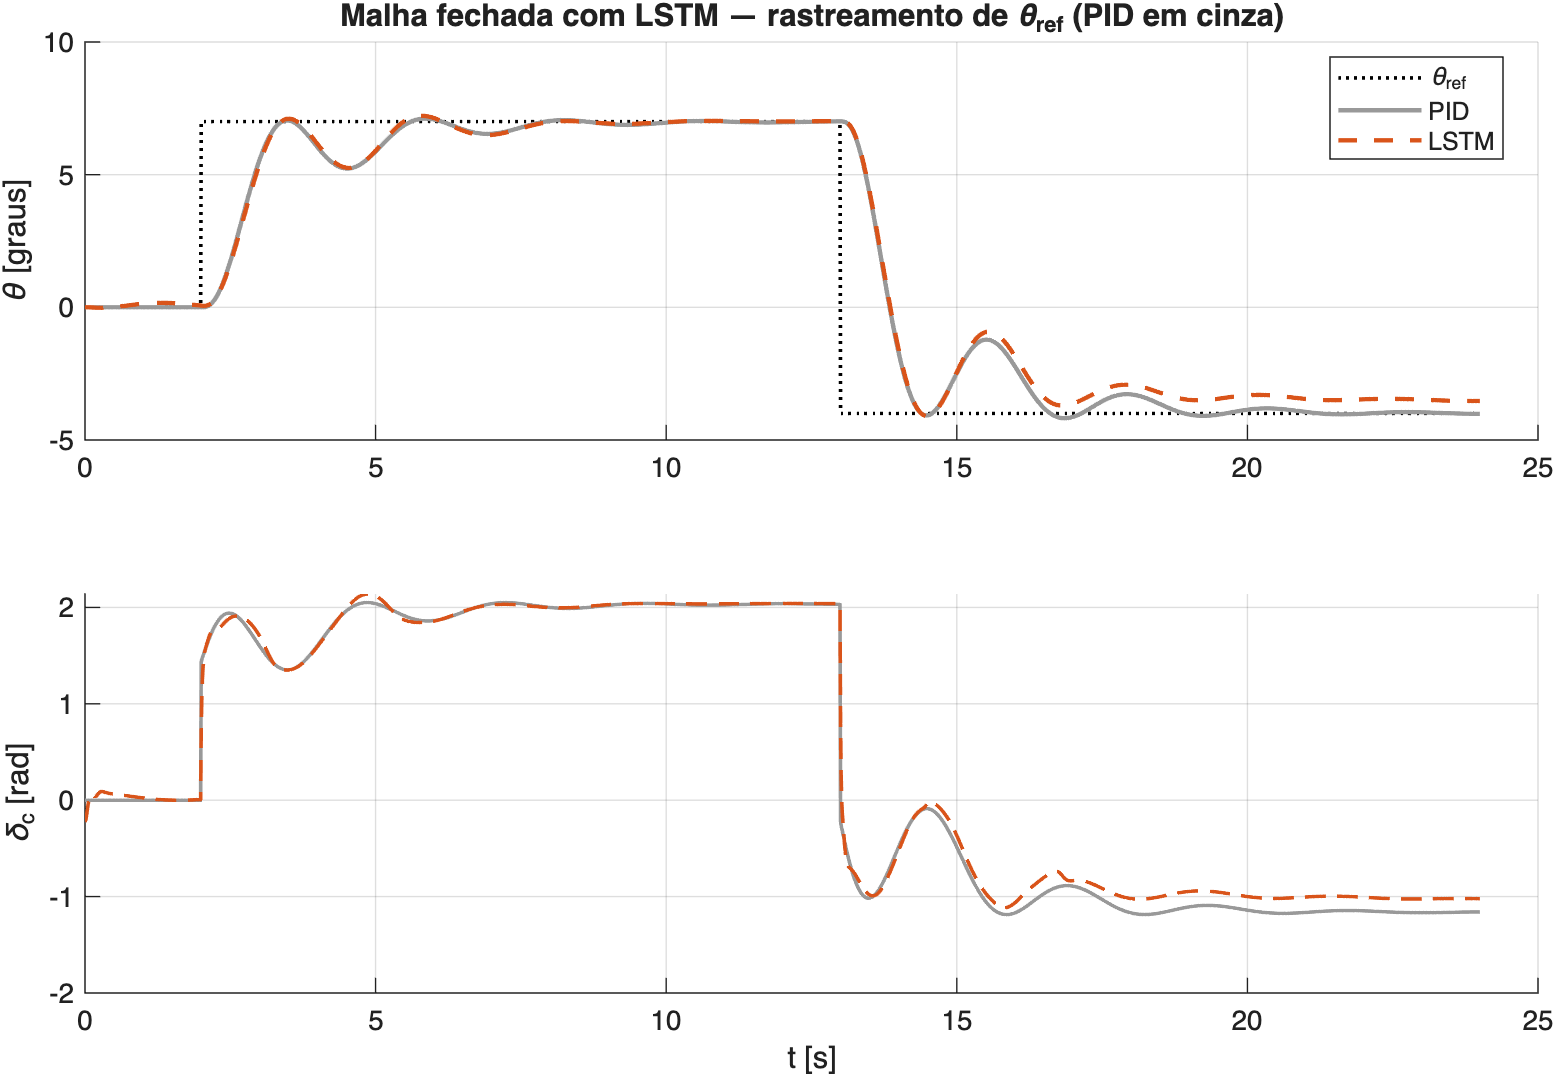
\includegraphics[width=0.84\textwidth]{malha_fechada_lstm.png}
  \caption{O mesmo avião comandado pela \textbf{rede neural} (em laranja), com o
  controlador clássico em cinza para comparação. As curvas quase se sobrepõem: a rede
  faz praticamente a mesma coisa que o controlador clássico.}
  \label{fig:lstm}
\end{figure}

A métrica de desempenho é o \textbf{RMSE de rastreamento} (raiz do erro quadrático médio
entre $\theta$ e $\thetaref$). A Tabela~\ref{tab:nominal} compara PID e LSTM em sete
cenários, incluindo perfis não vistos no treino. A LSTM empata com o PID (RMSE mediano
$0{,}91^\circ$ contra $0{,}92^\circ$), com desvio RMS entre as duas respostas de apenas
$0{,}13^\circ$ --- praticamente sobrepostas.

\begin{table}[H]
\centering
\caption{Comparação PID $\times$ LSTM em sete cenários. RMSE de rastreamento (entre
$\theta$ e $\thetaref$) e desvio RMS entre as duas respostas, em graus.
($^{\dagger}$ perfis não vistos no treino.)}
\label{tab:nominal}
\begin{tabular}{lccc}
\toprule
Cenário & \begin{tabular}{c}RMSE PID\\ (°)\end{tabular}
        & \begin{tabular}{c}RMSE LSTM\\ (°)\end{tabular}
        & \begin{tabular}{c}Desvio RMS\\ LSTM--PID (°)\end{tabular}\\
\midrule
degrau $+3^\circ$            & 0,47 & 0,49 & 0,13\\
degrau $+5^\circ$           & 0,79 & 0,79 & 0,08\\
degrau $+7^\circ$           & 1,10 & 1,11 & 0,05\\
degrau $-5^\circ$           & 0,79 & 0,80 & 0,18\\
dois degraus                & 0,92 & 0,92 & 0,19\\
rampa$^{\dagger}$           & 0,93 & 0,91 & 0,15\\
multisseno$^{\dagger}$      & 1,93 & 1,89 & 0,11\\
\midrule
\textbf{mediana}            & \textbf{0,92} & \textbf{0,91} & \textbf{0,13}\\
\bottomrule
\end{tabular}
\end{table}

A Figura~\ref{fig:nominal} mostra a situação ``subir $5^\circ$''. Vale destacar: foi
\emph{exatamente} este caso que, antes do treino extra (DAgger), ficava oscilando sem
parar. Depois do DAgger, a rede acompanha o controlador clássico perfeitamente.

\begin{figure}[H]
  \centering
  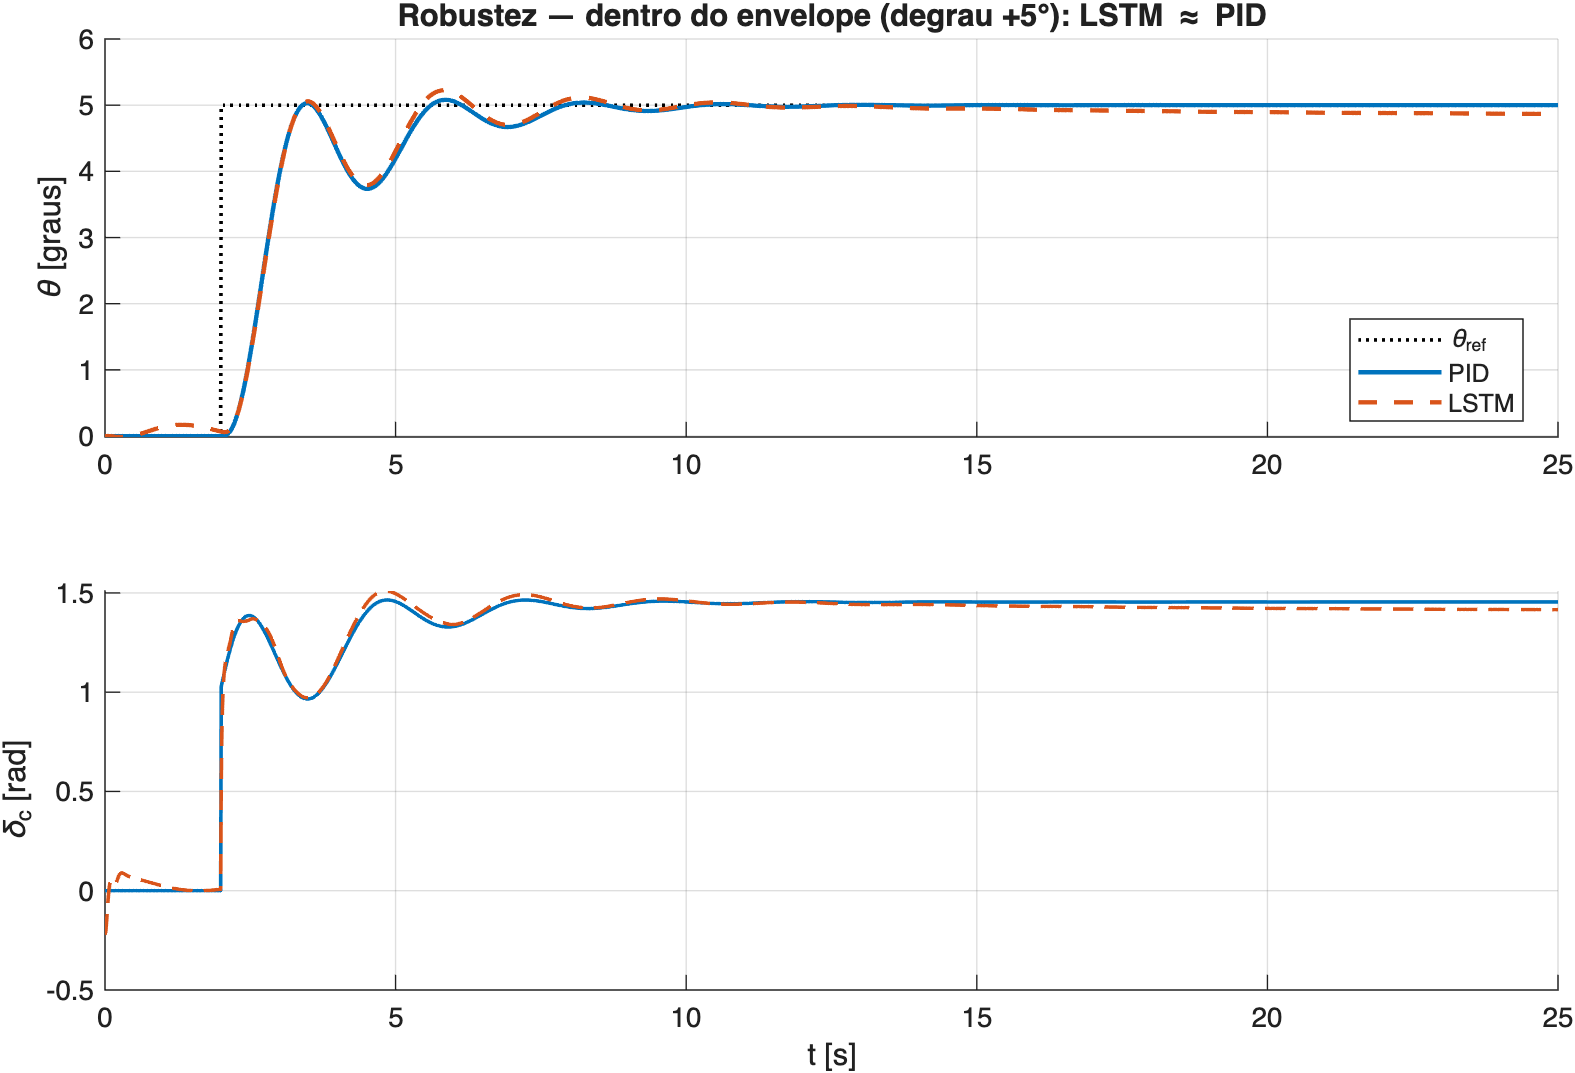
\includegraphics[width=0.84\textwidth]{rob_nominal.png}
  \caption{Subir $5^\circ$: rede neural (laranja) e controlador clássico (azul) são
  praticamente indistinguíveis. Antes do treino extra (DAgger), neste mesmo caso o
  avião ficava balançando $\pm3{,}5^\circ$ sem parar.}
  \label{fig:nominal}
\end{figure}

% =====================================================================
\section{Onde a rede falha: testando fora do que ela aprendeu}
% =====================================================================

A rede foi treinada em situações ``de rotina'': o avião começando nivelado e pedidos de
inclinação de até $10^\circ$. O que acontece quando saímos disso? Testamos, e a
resposta confirma a lição central: \textbf{a rede só é boa onde já viu situações
parecidas}. Importante: em \emph{todos} os testes, mesmo falhando, o avião nunca
descontrolou de vez --- a rede sempre se manteve estável.

\paragraph{(1) Começar fora da posição.} Se o avião já \emph{começa} inclinado (por
exemplo, $+8^\circ$) e pedimos que volte a zero, o controlador clássico faz isso de
forma suave. A rede também consegue voltar ao alvo --- mas com um começo \textbf{muito
agitado}, balançando bastante antes de se acalmar (Figura~\ref{fig:ci}). O motivo:
durante o treino, o avião \emph{sempre} começava nivelado; começar já inclinado é uma
situação nova, e a rede leva alguns segundos para ``se achar''.

\begin{figure}[H]
  \centering
  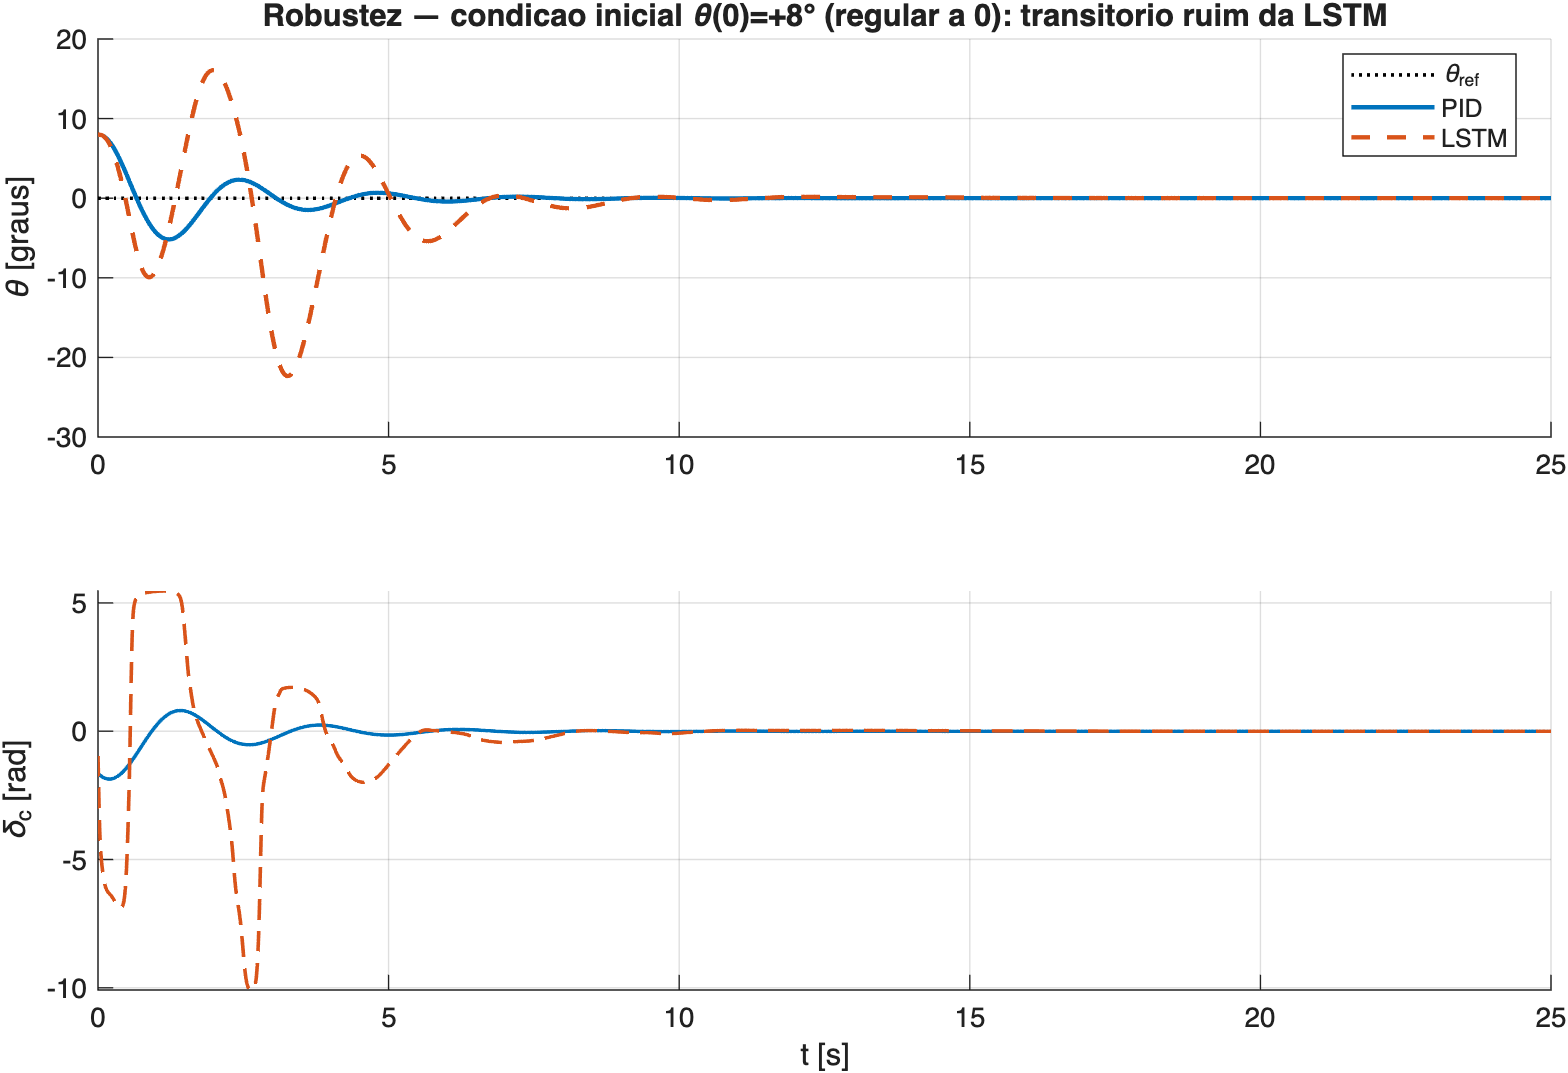
\includegraphics[width=0.84\textwidth]{rob_cond_inicial.png}
  \caption{Avião começando inclinado em $+8^\circ$ e tendo que voltar a zero. O
  controlador clássico (azul) volta suave; a rede neural (laranja) chega lá, mas com
  um início bem agitado, porque nunca treinou começando fora da posição.}
  \label{fig:ci}
\end{figure}

\paragraph{(2) Pedir inclinações maiores do que as do treino.} A rede treinou com
pedidos de até $10^\circ$. Quando pedimos $13^\circ$, ela \textbf{volta a oscilar} ---
o avião fica balançando em torno do alvo (Figura~\ref{fig:extrap}). O controlador
clássico, que não ``decora'' e sim segue uma fórmula, acomoda normalmente. Esse é o
limite mais claro da rede: fora da faixa que viu, ela falha.

\begin{figure}[H]
  \centering
  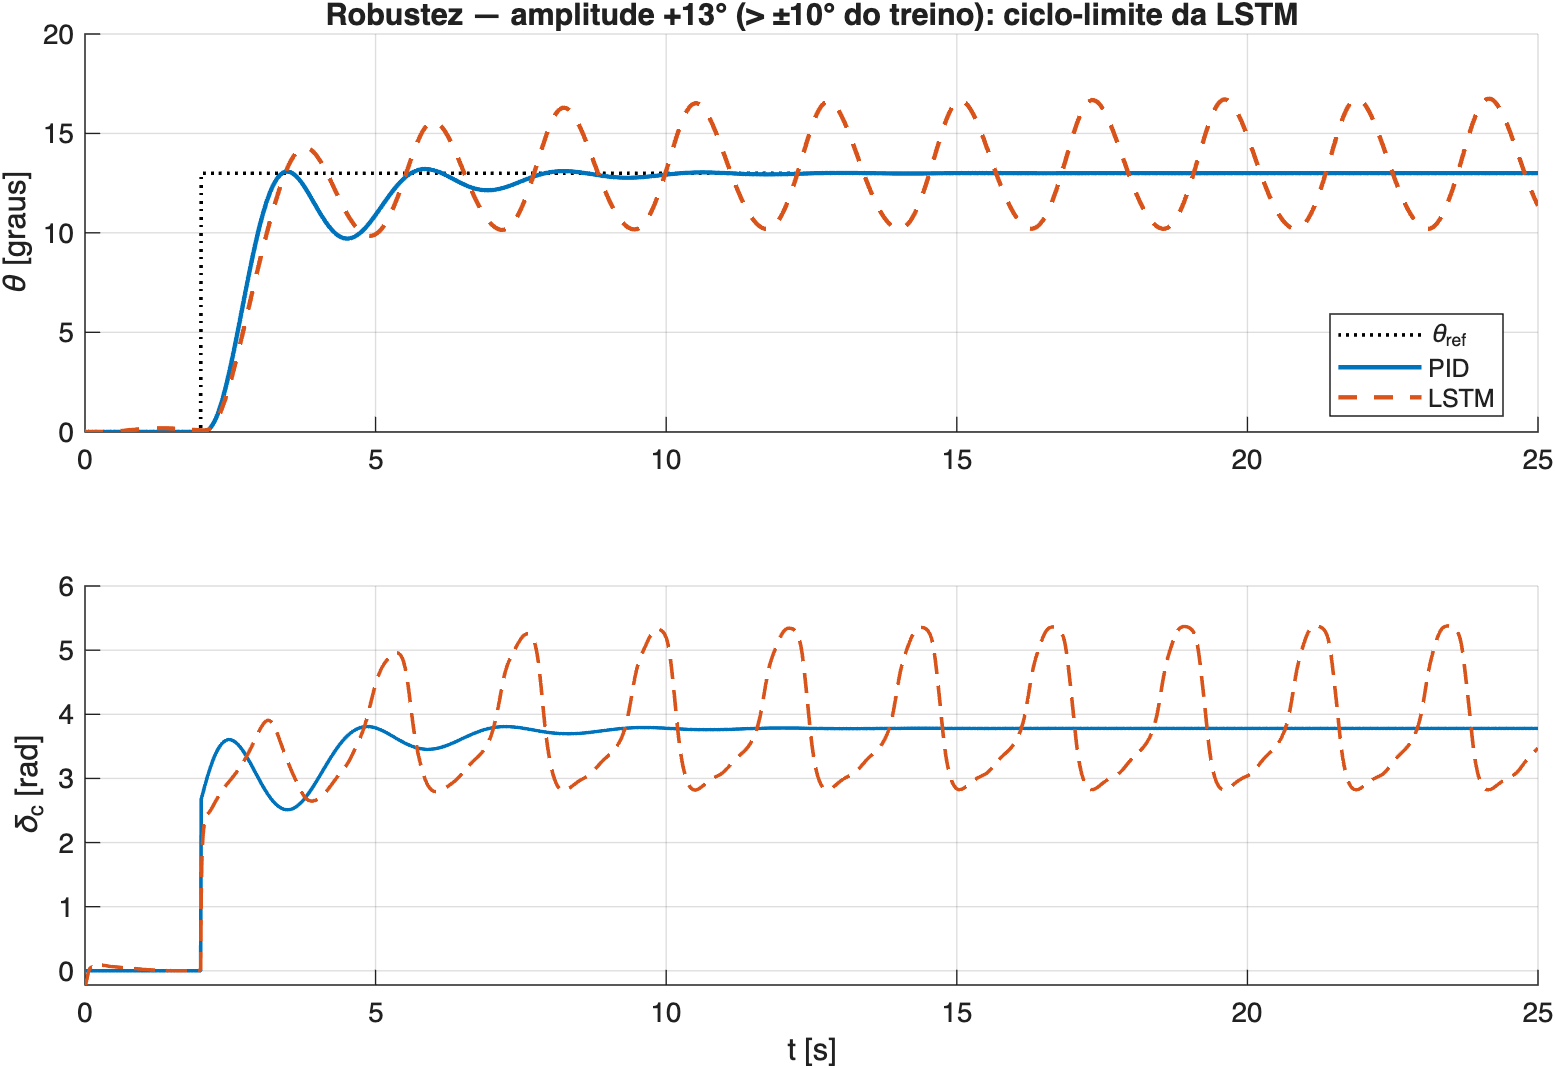
\includegraphics[width=0.84\textwidth]{rob_extrapolacao.png}
  \caption{Pedido de $13^\circ$ (acima dos $10^\circ$ que a rede viu no treino): o
  controlador clássico (azul) acomoda limpo; a rede neural (laranja) fica oscilando
  sem parar.}
  \label{fig:extrap}
\end{figure}

\paragraph{(3) Pedir movimentos mais rápidos.} Quando a inclinação desejada muda muito
rápido, \emph{os dois} controladores ficam para trás --- mas igualmente
(Figura~\ref{fig:rapida}). Aqui não é culpa da rede: é um limite físico do próprio
avião, que não consegue acompanhar mudanças tão rápidas. A rede continua imitando bem o
clássico.

\begin{figure}[H]
  \centering
  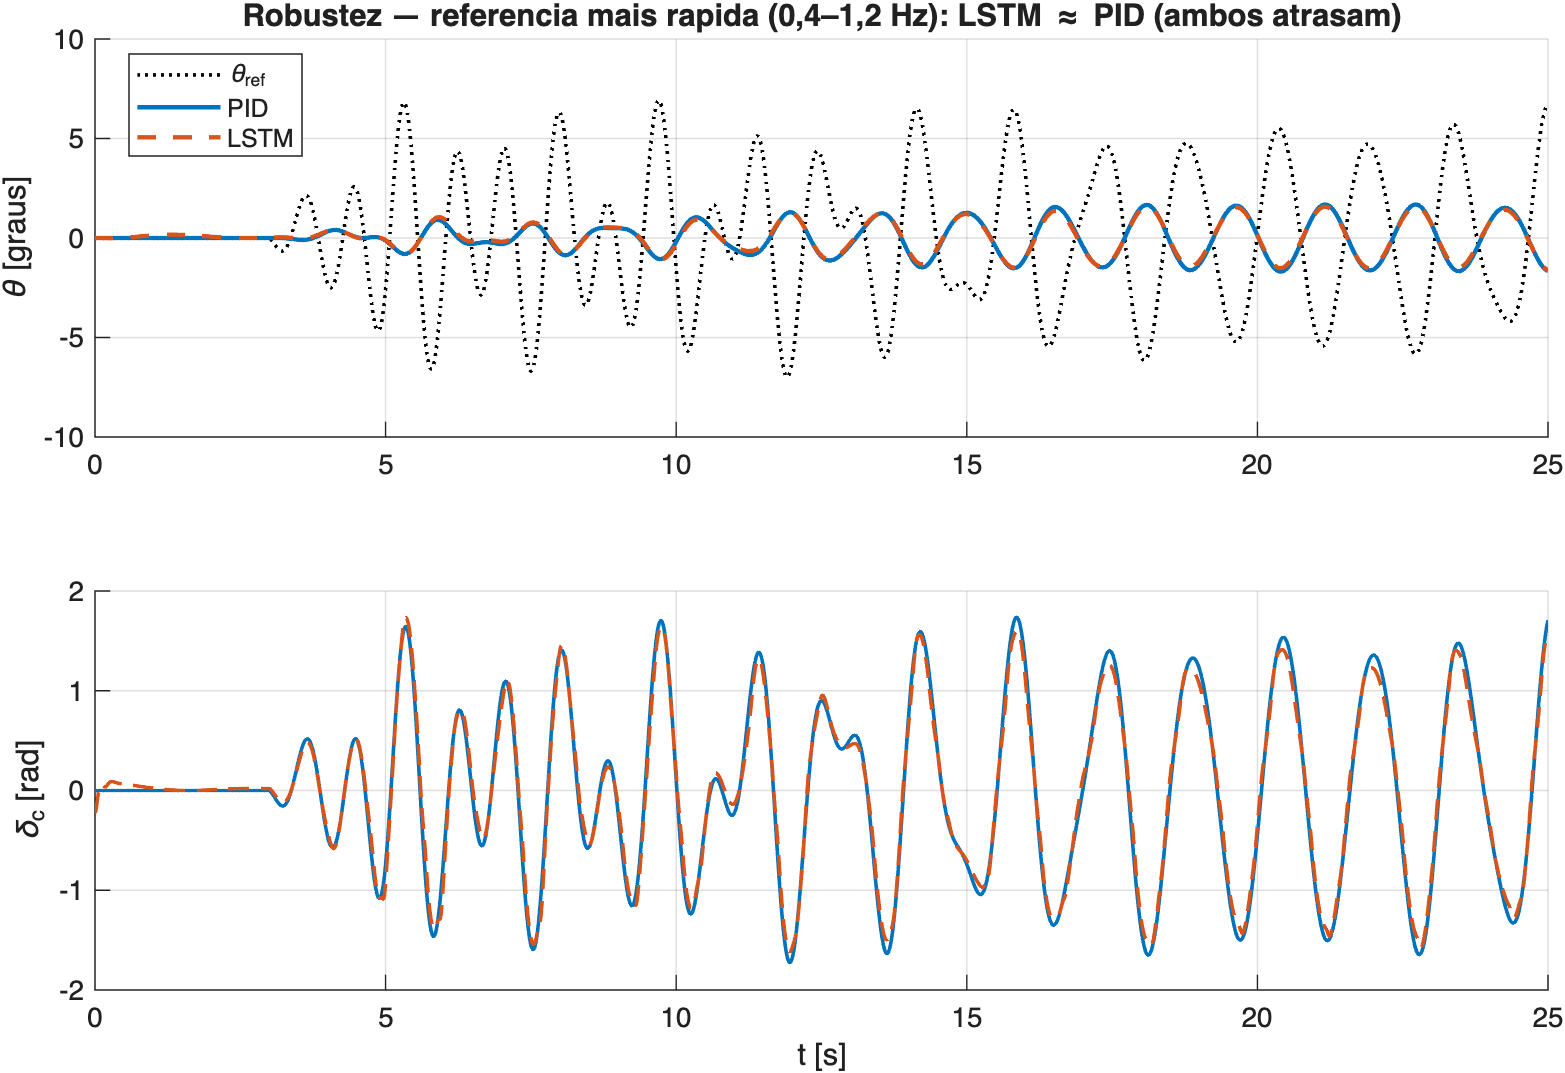
\includegraphics[width=0.84\textwidth]{rob_ref_rapida.png}
  \caption{Pedido que muda muito rápido: rede neural (laranja) e controlador clássico
  (azul) reagem quase igual --- ambos ``atrasam'' em relação ao alvo. É limite do
  avião, não da rede.}
  \label{fig:rapida}
\end{figure}

A Tabela~\ref{tab:robustez} resume. Note que em todos os casos o avião permaneceu
estável (não descontrolou).

\begin{table}[H]
\centering
\caption{Testes fora do envelope de treino (RMSE de rastreamento, em graus). Em todos os
casos a malha permaneceu estável.}
\label{tab:robustez}
\begin{tabular}{lccc}
\toprule
Cenário & \begin{tabular}{c}RMSE PID\\ (°)\end{tabular}
        & \begin{tabular}{c}RMSE LSTM\\ (°)\end{tabular} & Estável?\\
\midrule
$\theta(0)=+8^\circ$, $\thetaref=0$        & 1,30 & 4,90 & sim\\
$\theta(0)=+10^\circ$, $\thetaref=-5^\circ$ & 1,96 & 5,37 & sim\\
degrau $+13^\circ$ (extrapolação)          & 2,05 & 2,92 & sim\\
degrau $-15^\circ$ (extrapolação)          & 2,36 & 2,56 & sim\\
referência rápida (0,4--1,2~Hz)            & 4,08 & 4,03 & sim\\
\bottomrule
\end{tabular}
\end{table}

% =====================================================================
\section{O que pode ser melhorado}
\label{sec:melhorias}
% =====================================================================

Os testes da seção anterior apontam, com clareza, onde o método pode crescer. As
melhorias abaixo estão ordenadas da mais direta (e que resolveria a maior parte das
falhas observadas) à mais ambiciosa.

\begin{enumerate}
  \item \textbf{Ampliar o envelope de treino.} Quase todas as falhas vêm de a rede ser
        testada \emph{fora} do que viu. A correção é direta: gerar os dados também com
        o avião \textbf{começando inclinado} ($\theta(0)\neq0$), com \textbf{amplitudes
        maiores} que $\pm10^\circ$ e com \textbf{referências mais rápidas}; em seguida,
        repetir o DAgger. A planta de simulação já permite começar fora da posição, então
        esse passo é barato e deve eliminar tanto a oscilação em ângulos grandes
        (Fig.~\ref{fig:extrap}) quanto boa parte do transitório agitado ao iniciar
        deslocado (Fig.~\ref{fig:ci}).

  \item \textbf{Resolver o ``arranque a frio'' da memória.} O pior caso --- começar
        inclinado --- piora porque o estado interno $h$ da LSTM (Eq.~\eqref{eq:lstm-ss})
        sempre \emph{parte do zero}, como se a rede ``acordasse'' sem saber em que
        situação o avião está. Além de treinar com $\theta(0)\neq0$, poder-se-ia
        \textbf{informar a inclinação inicial à rede} (como uma entrada extra) ou dar a
        ela um breve intervalo de ``aquecimento'' antes de assumir o comando.

  \item \textbf{Adicionar uma camada de segurança (supervisor).} Como a rede não tem
        garantia fora do envelope, um esquema prático é \textbf{monitorar} se a situação
        atual está dentro da faixa conhecida e, em caso negativo, \textbf{devolver o
        comando ao PID} (ou limitar/saturar a ação da rede). Assim combina-se o melhor
        dos dois mundos: a rede onde ela é boa, e a garantia clássica como rede de
        proteção.

  \item \textbf{Testar robustez a variações da planta.} Toda a avaliação usou um
        \emph{único} modelo de avião. Na prática, massa, velocidade e centro de
        gravidade mudam. Convém verificar como a rede se comporta quando os parâmetros da
        planta variam --- e, se necessário, treiná-la com uma \emph{família} de plantas
        (treino com variação), algo que o controlador clássico tolera por projeto.

  \item \textbf{Incluir ruído de sensor.} Os dados de treino são ``limpos''. Medidas
        reais de $\theta$ têm ruído; treinar com ruído (e talvez penalizar comandos muito
        ``nervosos'') tornaria a rede mais realista e suave.

  \item \textbf{Buscar garantias formais de estabilidade.} A diferença de fundo para o
        PID é que este tem \textbf{prova matemática} de estabilidade, e a rede não.
        Existem técnicas recentes para \emph{certificar} controladores neurais (análise
        por funções de Lyapunov, restrições integrais quadráticas / IQC, verificação
        formal de redes). Aplicá-las aqui transformaria a ``garantia na prática'' numa
        garantia de fato --- um próximo passo natural e de maior fôlego.

  \item \textbf{Enxugar a rede.} Para embarcar em hardware real, valeria estudar redes
        menores ou alternativas (por exemplo \emph{GRU}, uma variante mais simples da
        LSTM) e técnicas de compressão, medindo o \emph{trade-off} entre tamanho e
        qualidade do controle.
\end{enumerate}

% =====================================================================
\section{Conclusão}
% =====================================================================

Principais conclusões deste estudo:

\begin{itemize}
  \item \textbf{Dá para trocar o controlador clássico por uma rede neural} e obter o
        mesmo desempenho --- desde que a rede seja treinada do jeito certo.
  \item \textbf{Só copiar o professor não é suficiente.} A rede parecia ótima ``no
        papel'', mas balançava o avião quando assumia o comando. O treino extra
        (DAgger), em que ela aprende com os próprios erros, resolveu isso.
  \item \textbf{A rede só é confiável no que já viu.} Dentro da faixa de treino, ela
        empata com o clássico. Fora dela --- começando muito inclinada ou com pedidos
        maiores --- ela piora, embora sem descontrolar. O controlador clássico, por
        seguir uma fórmula, não tem esse limite.
\end{itemize}

A diferença essencial é essa: o controlador clássico tem \textbf{garantia matemática}
de funcionar em qualquer situação; a rede neural tem apenas \textbf{garantia na
prática}, e só onde foi treinada. Para ampliar essa faixa, bastaria treinar a rede
também em situações mais variadas (começando inclinada, com pedidos maiores) e repetir
o DAgger --- o que mostraria, na prática, que o limite observado é de \emph{falta de
exemplos}, não do método.

\textbf{Em resumo:} uma rede neural pode, sim, substituir um controlador clássico de
avião com a mesma qualidade --- contanto que a gente treine direito e respeite o seu
limite: ela é tão boa quanto os exemplos que viu.

% =====================================================================
\begin{thebibliography}{9}\small
% =====================================================================

\bibitem{ross2011} S.~Ross, G.~Gordon, J.~A.~Bagnell.
\emph{A Reduction of Imitation Learning and Structured Prediction to No-Regret Online
Learning} (DAgger). \emph{Proceedings of AISTATS}, 2011.

\bibitem{espin2024} J.~Espin, D.~Zhang, D.~Toti, A.~Pozzi.
\emph{Deep-MPC: A DAGGER-Driven Imitation Learning Strategy for Optimal Constrained
Battery Charging}. arXiv:2406.15985, 2024.

\bibitem{hochreiter1997} S.~Hochreiter, J.~Schmidhuber.
\emph{Long Short-Term Memory}. \emph{Neural Computation}, 9(8):1735--1780, 1997.

\bibitem{nguyen2016} K.~Nguyen.
\emph{Imitation Learning with Recurrent Neural Networks}. arXiv:1607.05241, 2016.

\end{thebibliography}

\end{document}
